\documentclass[11pt,fleqn,a4paper]{scrartcl}
\binoppenalty=1000
\relpenalty=1000
\usepackage[utf8]{inputenc}
\usepackage[unicode, pdftex,pdfborder=0 0 0,colorlinks, linkcolor=black]{hyperref}
\usepackage[english,russian]{babel}
\usepackage{indentfirst}
\usepackage{booktabs}
\usepackage{misccorr}
\usepackage{graphicx}
\usepackage{multirow}
\usepackage{tikz}
\usepackage{amsmath}
\usepackage{wrapfig}
\usepackage{longtable}
\usepackage{algorithm2e}
\begin{document}

\begin{center}
Moscow STATE UNIVERSITY \\ named after M. V. LOMONOSOV\\ Faculty of mechanics and mathematics
\end{center}
\begin{figure}[htbp]
\centering
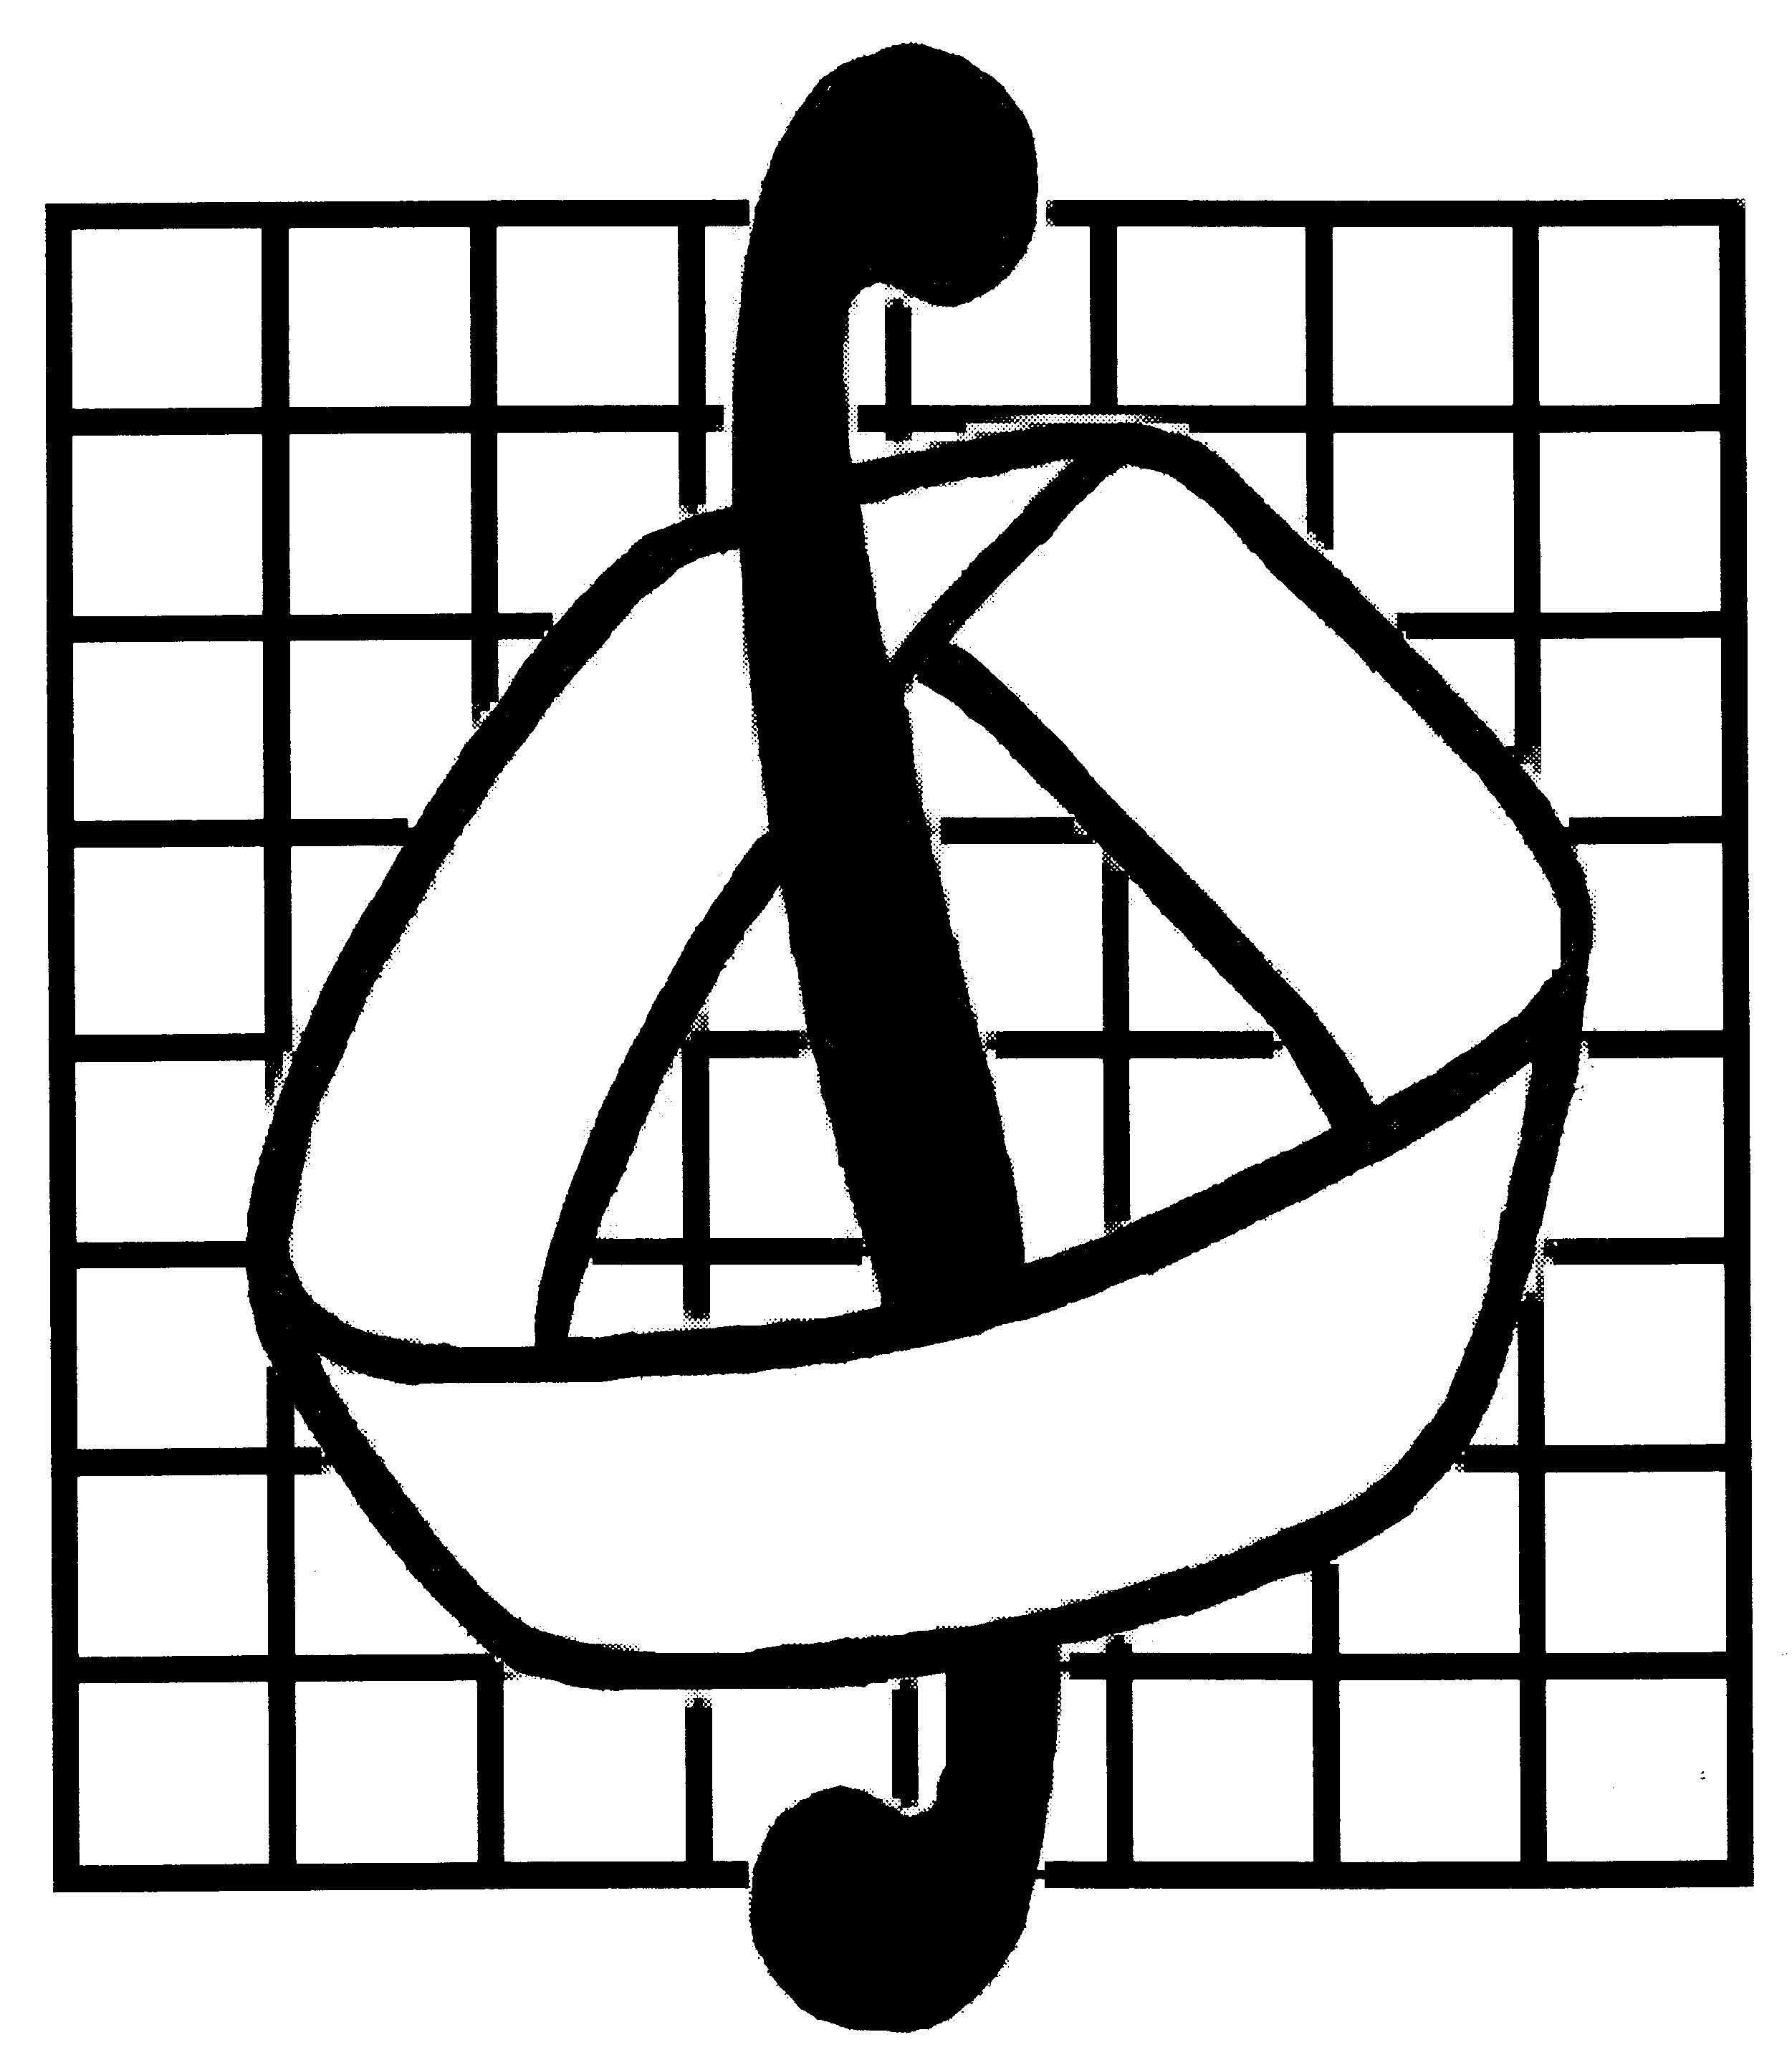
\includegraphics[width=0.3\textwidth]{36cacac6.png}
\end{figure}
\begin{center}
\textbf{\large{\textit{Coursework.}}}
\end{center}
\textbf{\large{\textit{Approximation of a polyhedron by a set of spatial segments. Building a polyhedron from a set of half-spaces.}}} \\
\begin{flushright} {Supervisor: V. D. Valedinsky\\ }\end{flushright}
\begin{flushright} {Student: M. N. Kovalkov\\ }\end{flushright}
\newpage
\tableofcontents
\newpage
\section{The problem of approximation of a polyhedron by a set of spatial segments.}
\subsection{Problem statement.}
There is a polyhedron and a set of target edges. It is assumed that the polyhedron is constructed inaccurately, and the target edges are accurate. You need to change the polyhedron so that it best matches the target edges.
\begin{center}
\begin{tabular}{cc}

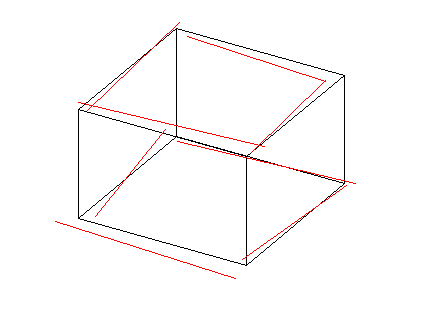
\includegraphics[width=0.5\textwidth]{input.png} &
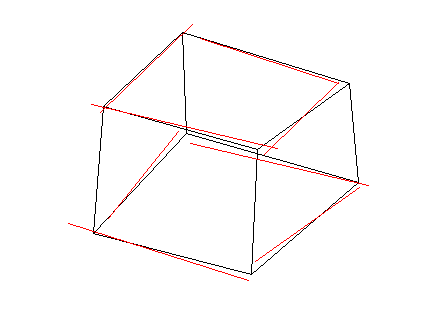
\includegraphics[width=0.5\textwidth]{out.png} \\
The original polyhedron& The modified polyhedron \\
\\
\end{tabular}
\end{center}
\subsection{Mathematical formalization of the problem. Build minimaliseren functionality}
There is a polyhedron $M$ defined by sets of its faces, edges, and vertices.
$$
\begin{cases}
p_{i}=(x_{i},y_{i},z_{i})- &\text{Coordinates of the polyhedron vertices,} i=\overline{1,n_{1}} \\
e_{j}=(a_{j, 1}, a_{j, 2}) - & \begin{array}[c]{ll}%
\text{Numbers of vertexes that are}
\\
\text{edge ends } e_{j} \text {,} j=\overline{1,n_{2}}
\end{array}\\
f_{k}=[b_{k,1}, \ldots, b_{k,m_{k}}] - & \text{Numbers of edges included in the face } f_{k} \text {,} k=\overline{1,n_{3}} \\
\end{cases}
$$
There is a list of target edges that are considered accurate and that correspond to the original edges of the polyhedron.
$$
\widetilde{e_{i}}=
\begin{cases}
(a_{i, x},a_{i, y},a_{i, z}), (b_{i, x}, b_{i, y},b_{i,z}) -
\text{coordinates of the two ends of this target edge. } \\
ind_{i}-
\text{number of the source edge,
which corresponds to the I-th target edge. }
\end{cases}
$$
\par
If there is no element for the current edge in the list of target edges, we assume that it is a target for itself. However, the weight with which it is included in the functional will be equal to $\omega_{i}=0.1$, while for a full target edge $\omega_{i}=1$. After expanding the list of target edges in the specified way, we assume that $\widetilde{e_{i}}$is the target edge corresponding to the original edge $e_{i}$ of the polyhedron $M$.\par
Do the edges of a polyhedron "movable", for this we introduce variables $\tilde p_{i,1}=(\tilde x_{i,1},\tilde y_{i,1},\tilde z_{i,1}),\tilde p_{i,1}=(\tilde x_{i,2},\tilde y_{i,2},\tilde z_{i,2}) $ corresponding to ends of "moving" edges. We want to find a configuration so that these edges are the least distant from their corresponding targets. To do this, we must deliver a minimum of the following functionality:
$$\sum_{i=1}^{n_{2}}\omega_{i}(\rho^{2}(\tilde p_{i,1},\widetilde{e_{i}})+\rho^{2}(\tilde p_{i, 2},\widetilde{e_{i}}))\rightarrow \min , \text{ where}$$
$\rho(\tilde p_{i,j},\widetilde{e_{i}})$-the distance between the ends of the "movable" edge and the line defined by the corresponding target edge.
\begin{figure}[htbp]
\centering
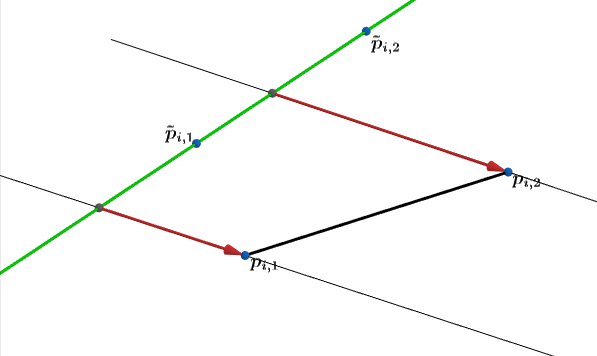
\includegraphics[width=0.7\textwidth]{distancce.png}
\end{figure}
\subsection{Calculating the distance from a point to a straight line.}
To calculate the distance, use the formula for calculating the projection of the vector $\overrightarrow{a}$ on the vector $\overrightarrow{b}$: \\
\begin{wrapfigure}[8]{r}{0.15\linewidth}
\begin{tikzpicture}
\coordinate [label=1:$L_{1}$] (A) at (0,0);
\coordinate [label=2:$L_{2}$] (B) at (1,3);
\coordinate [label=3:$P$](C) at (1.8,1.4);
\coordinate [label=4:$P'$](D) at (0.6,1.8);
\draw [->,black] (A) -- (B);
\draw [->,black] (A) -- (C);
\draw [red] (C) -- (D);
\draw [->,black] (A) -- (D);
\end{tikzpicture}
\end{wrapfigure}
$$pr_{\overrightarrow{L_{1}L_{2}}} \overrightarrow{L_{1}P}=\frac{( \overrightarrow{L_{1}P}, \overrightarrow{L_{1}L_{2}})}{ (\overrightarrow{L_{1}L_{2}}, \overrightarrow{L_{1}L_{2}})} \overrightarrow{L_{1}L_{2}},\text{ where}$$ ( * ,*) -- standard scalar product:
$$( \overrightarrow{a}, \overrightarrow{b})=a_{x}b_{x}+a_{y}b_{y}+a_{z}b_{z}$$
Then we use the Pythagorean theorem to calculate the distance:

$$\rho^{2}(P,L_1L_2)=|\overrightarrow{L_{1}P}|^{2}-|pr_{\overrightarrow{L_{1}L_{2}}} \overrightarrow{L_{1}P}|^{2}=\frac{(\overrightarrow{L_{1}P},\overrightarrow{L_{1}P})(\overrightarrow{L_{1}L_{2}},\overrightarrow{L_{1}L_{2}})-(\overrightarrow{L_{1}P},\overrightarrow{L_{1}L_{2}})(\overrightarrow{L_{1}P},\overrightarrow{L_{1}L_{2}})}{(\overrightarrow{L_{1}L_{2}},\overrightarrow{L_{1}L_{2}})}$$

\subsection{Proof of convexity of the functional.}
For correct application of the inner point method, the convexity of the minimalized functional is required. We prove that the functional we are considering is convex.
Let's consider one summand of the sum that forms our functional:
$$
F=(x-a_{x})^{2}+(y-a_{y})^{2}+(z-a_{z})^{2}-\frac{((x-a_{x})(b_{x}-a_{x})+(x-a_{y})(b_{y}-a_{y})+(x-a_{z})(b_{z}-a_{z}))^{2}}{(b_{x}-a_{x})^2+(b_{y}-a_{y})^2+(b_{z}-a_{z})^2}
$$
We introduce the notation: $c_{1}:=(b_{x}-a_{x}),c_{2}:=(b_{y}-a_{y}),c_{3}:=(b_{z}-a_{z}),c:=c_{1}^{2}+c_{2}^{2}+c_{3}^{2}$.\\ And write the matrix of second partial derivatives $F$:
$$
\begin{pmatrix}
\frac{\partial^{2}F}{\partial x^{2}} & \frac{\partial^{2}F}{\partial x \partial y} & \frac{\partial^{2}F}{\partial x \partial z} \\
\frac{\partial^{2}F}{\partial y \partial x} & \frac{\partial^{2}F}{\partial y^{2}} & \frac{\partial^{2}F}{\partial y \partial z} \\
\frac{\partial^{2}F}{\partial z\partial x} & \frac{\partial^{2}F}{\partial z \partial y} & \frac{\partial^{2}F}{\partial z^{2}} \\
\end{pmatrix}
=
\begin{pmatrix}
2(1-\frac{c_{1}^{2}}{c}) & -\frac{c_{1}c_{2}}{c} & -\frac{c_{1}c_{3}}{c}\\
-\frac{c_{1}c_{2}}{c}& 2(1-\frac{c_{2}^{2}}{c}) & -\frac{c_{2}c_{3}}{c}\\
-\frac{c_{1}c_{3}}{c}& -\frac{c_{2}c_{3}}{c} & 2(1-\frac{c_{3}^{2}}{c}) \\
\end{pmatrix}
$$
Let's check the matrix for nonnegative certainty using the Sylvester Criterion. To do this, we calculate the determinants of major minors.\\
1)$|\Delta_{1}|=2\frac{c_{2}^{2}+c_{3}^{2}}{c}\geq 0$\\
2)$|\Delta_{2}|
=
\begin{vmatrix}
2(1-\frac{c_{1}^{2}}{c}) & -\frac{c_{1}c_{2}}{c} \\
-\frac{c_{1}c_{2}}{c}& 2(1-\frac{c_{2}^{2}}{c}) \\
\end{vmatrix}=
4-4\frac{c_{1}^{2}+c_{2}^{2}}{c}+4\frac{c_{1}^{2}c_{2}^{2}}{c^{2}}-\frac{c_{1}^{2}c_{2}^{2}}{c^{2}}=4\frac{c_{3}^{2}}{c}+3\frac{c_{1}^{2}c_{2}^{2}}{c^{2}}\geq 0
$\\
3) $|\Delta_{3}|=
\begin{vmatrix}
2(1-\frac{c_{1}^{2}}{c}) & -\frac{c_{1}c_{2}}{c} & -\frac{c_{1}c_{3}}{c}\\
-\frac{c_{1}c_{2}}{c}& 2(1-\frac{c_{2}^{2}}{c}) & -\frac{c_{2}c_{3}}{c}\\
-\frac{c_{1}c_{3}}{c}& -\frac{c_{2}c_{3}}{c} & 2(1-\frac{c_{3}^{2}}{c}) \\
\end{vmatrix}=
8(1-\frac{c_{1}^{2}}{c})(1-\frac{c_{2}^{2}}{c})(1-\frac{c_{3}^{2}}{c})-2\frac{c_{1}^{2}c_{2}^{2}c_{3}^{2}}{c^{3}}- \\ -
2\frac{c_{1}^{2}c_{3}^{2}}{c^{2}}(1-\frac{c_{2}^{2}}{c})-2\frac{c_{2}^{2}c_{3}^{2}}{c^{2}}(1-\frac{c_{1}^{2}}{c})
-\frac{c_{1}^{2}c_{2}^{2}}{c^{2}}(1-\frac{c_{3}^{2}}{c})= 8 - 4\frac{c_{1}^{2}c_{2}^{2}c_{3}^{2}}{c^{3}}+6(\frac{c_{1}^{2}c_{2}^{2}}{c^{2}}+\frac{c_{1}^{2}c_{3}^{2}}{c^{2}}+\frac{c_{2}^{2}c_{3}^{2}}{c^{2}})-8\frac{c_{1}^{2}+c_{2}^{2}+c_{3}^{2}}{c}= \\ =6(\frac{c_{1}^{2}c_{2}^{2}}{c^{2}}+\frac{c_{1}^{2}c_{3}^{2}}{c^{2}})+2(\frac{c_{2}^{2}c_{3}^{2}}{c^{2}})+4+\frac{c_{2}^{2}c_{3}^{2}}{c^{2}}(1-\frac{c_{1}^{2}}{c})=6(\frac{c_{1}^{2}c_{2}^{2}}{c^{2}}+\frac{c_{1}^{2}c_{3}^{2}}{c^{2}})+2(\frac{c_{2}^{2}c_{3}^{2}}{c^{2}})+4+\frac{c_{2}^{2}c_{3}^{2}}{c^{2}}(\frac{c_{2}^{2}+c_{3}^{2}}{c})\geq 0
$\\
Thus, we have shown that the matrix of the second partial derivatives of the function is non-negative, hence this function is convex. It remains to remember that the sum of convex functions is also convex (a Direct consequence of the definition via Jensen's inequality).\par
Thus, the convexity of the problem and, as a result, the correctness of using the inner point method for its solution is shown.
\subsection{Conditions imposed on the functionality.}
A number of restrictions must be imposed on the functionality, the main of which is the following: if the original edges lay in the same face, then the "moving" edges must lie in the same face. In other words:
$$
\forall k=\overline{1,n_{3}} \text{ } \exists \text{ плоскость } \pi_{k} : \forall j \in f_{k}, \overline{\tilde{p}_{j,1},\tilde{p}_{j,2}} \in \pi_{k}
$$

Mathematically, you can use the determinant to write the condition that 4 points belong to the same plane:
$$\begin{vmatrix}
x_2-x_1 && y_2-y_1&& z_2-z_1 \\
x_3-x_1 && y_3-y_1&& z_3-z_1 \\
x_4-x_1 && y_4-y_1&& z_4-z_1 \\
\end{vmatrix}=0$$

Accordingly, for n points, this condition will look like this:
$$
\begin{cases}
\begin{vmatrix}
x_2-x_1 && y_2-y_1&& z_2-z_1 \\
x_3-x_1 && y_3-y_1&& z_3-z_1 \\
x_4-x_1 && y_4-y_1&& z_4-z_1 \\
\end{vmatrix}=0 \\
\newline \\
\begin{vmatrix}
x_2-x_1 && y_2-y_1&& z_2-z_1 \\
x_3-x_1 && y_3-y_1&& z_3-z_1 \\
x_5-x_1 && y_5-y_1&& z_5-z_1 \\
\end{vmatrix}=0 \\
\hdots \hdots \hdots \hdots \hdots \hdots \hdots \hdots \hdots \hdots \hdots \\
\begin{vmatrix}
x_2-x_1 && y_2-y_1&& z_2-z_1 \\
x_3-x_1 && y_3-y_1&& z_3-z_1 \\
x_n-x_1 && y_n-y_1&& z_n-z_1 \\
\end{vmatrix}=0 \\
\end{cases}
$$
\begin{figure}
\centering
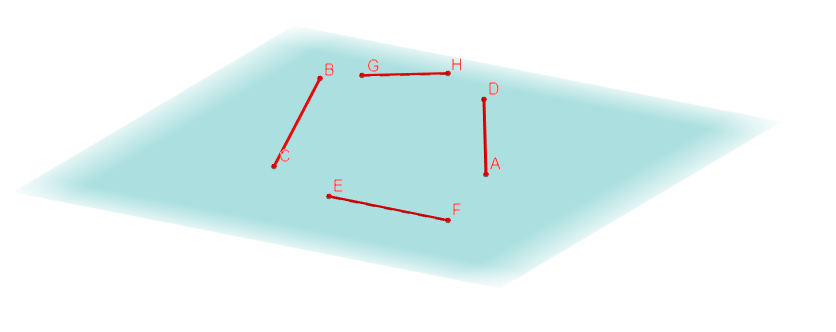
\includegraphics[width=0.7\textwidth]{inoneplane.png}
\end{figure}
However, this method of writing is quite cumbersome and, in addition, gives "cubic" conditions imposed on the problem. On the other hand, you can enter new variables $A_{k}, B_{k},C_{k},D_{k}, \forall k=\overline{1,n_{3}}$-coefficients from the equations of the planes. They do not participate in writing the minimalized functional, but they can be used to write the conditions of belonging to a single face quite simply:
$$
\begin{cases}
A_{k}\tilde{x}_{j,1}+B_{k}\tilde{y}_{j,1}+C_{k}\tilde{z}_{j,1}+D_{k}=0, \forall j \in f_{k}
\\
A_{k}\tilde{x}_{j, 2}+B_{k}\tilde{y}_{j, 2}+C_{k}\tilde{z}_{j, 2}+D_{k}=0, \forall j \in f_{k}
\\
A_{k}^{2}+B_{k}^{2}+C_{k}^{2}=1-\text{ coefficient normalization}
\end{cases}
$$
\begin{wrapfigure}[14]{r}{0.25\linewidth}

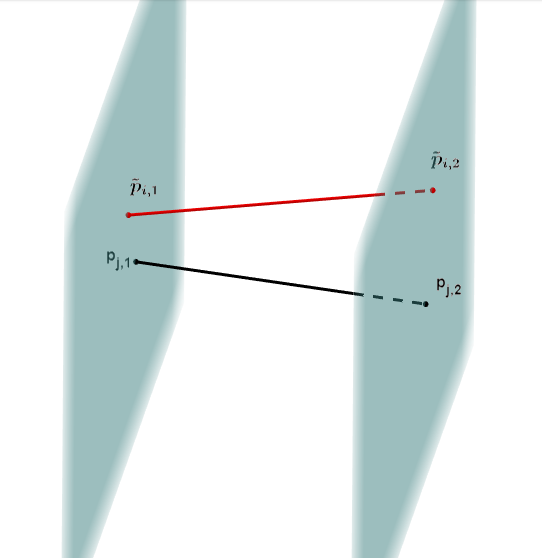
\includegraphics[width=0.4\textwidth]{innormalplane.png}
\end{wrapfigure}
\par
Equally important are the conditions for the ends of the "moving" edges to belong to the normal planes of the original edges of the polyhedron (non-target). They can be written as follows:
$$
\begin{cases}
\tilde{p}_{j,1} \in N(p_{e_{j}[1]},e_{j})\\
\tilde{p}_{j,2} \in N(p_{e_{j}[2]},e_{j})
\end{cases}
$$
where $N(p, e)$is a plane normal to the vector $e$ and passing through the point $p$.\par
These conditions are necessary to prevent the mobile edges from running away.
\section{Building a polyhedron from a set of half-spaces.}
After solving the optimization problem, we have sets of moving edges and the planes in which they lie. However, we would like to use this data to construct a polyhedron. The algorithm described below will help you solve this problem.
\par
To begin with, we get half-spaces from a set of planes. To do this, we calculate the center of mass of the original polyhedron and substitute it in the equations of planes. if we get a positive number, then the plane is given by the internal normal, so we multiply the coefficients of the plane by -1. Now we have a set of half-spaces whose intersection is the desired polyhedron.
\par
Let's go to the algorithm for constructing a polyhedron based on a set of half-spaces:
\begin{algorithm}[H]

x=1\;
cub=createCub(x)\;
\While{ True}{
oldFacets=cub.facets\;
\For{plane $\in$ planes}
{
newFacet=$\varnothing$\;
newEdges=$\varnothing$\;
\For{facet $\in$ cub.facets}
{
newPoints=$\varnothing$\;
\For{ edge $\in$ facet.edges}
{
\If{edge $\cap$ plane $\neq \varnothing$}
{
newPoints=newPoints $\cup$ (edge $\cap$ plane)\;
}
reconstructEdge(edge)\;
}
reconstructFacet(facet)\;
newEdges=newEdges $\cup$ edgeConstruct(newPoints)
}
newFacet=facetConstruct(newEdges)\;
cub.facets=cub.facets $\cup$ newFacet\;
}
\eIf{cub.facets $\cap$ oldFacets =$\varnothing$}
{
break\;
}
{
x=2x\;
cub=createCub(x)\;
}
}

\end{algorithm}
\begin{wrapfigure}[15]{r}{0.4\linewidth}

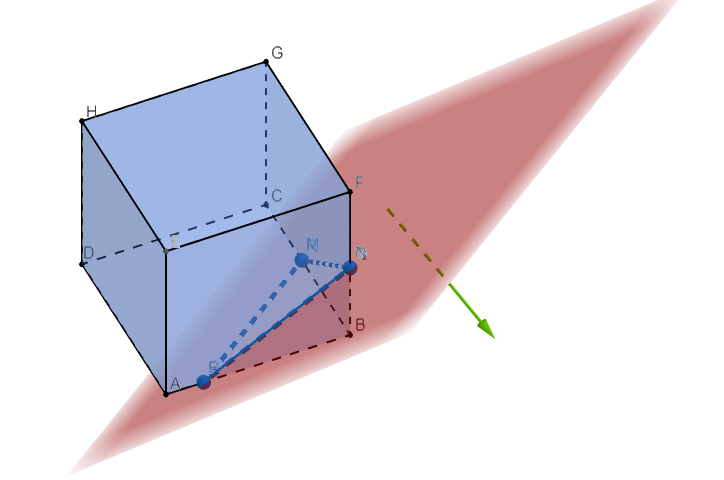
\includegraphics[width=0.6\textwidth]{cub3.png}
\end{wrapfigure}
Initially, we create an enclosing cube, from which we will cut off half-spaces. Let's describe the procedure for clipping a plane from a cube. We go through all the faces of the enclosing cube and in each face we look at the intersection of all the edges of this face with the plane being cut off. After getting the intersection points, we change the edges (taking only the part of the edge that lies in the desired half-space) and add the edge to the face. Edges that lie entirely in the opposite half-space are deleted. By memorizing the intersection edges, we form a new face of the enclosing cube (now it is no longer a cube, but an enclosing polyhedron) and add it to its structure. By doing this with the entire list of half-spaces, we get a polyhedron. However, the original enclosing cube may have been too small, so if a part of the face of the original enclosing cube remains in the polyhedron after the intersection of the half-spaces, then we double its size and start the process again.
\par
It should be noted that the algorithm requires consideration of a large number of extreme cases: intersections along a vertex, edge, or plane.

\section{Tools for software implementation of the task.}
\subsection{IPOPT}
The inner point method is implemented in the IPOPT library. Let's describe the installation process for this library.
\begin{enumerate}
\item Download the library from the repository:
\begin{verbatim}
$ svn co https://projects.coin-or.org/svn/Ipopt/stable/3.12 CoinIpopt
\end{verbatim}
\item Go to the folder with the IPOPT distribution:
\begin{verbatim}
$ cd CoinIpopt
\end{verbatim}
\item Download the third-party libraries needed to build IPOPT:
\begin{verbatim}
$ cd /ThirdParty/Blas
$ ./get.Blas 
$ cd ..
$cd Lapack 
$ ./get.Lapack 
$ cd ..
$cd ASL 
$ ./get.ASL
etc for all folders in ThirdPart
\end{verbatim}
\item Creating the build directory:
\begin{verbatim}
$ mkdir build
\end{verbatim}
and go to it:
\begin{verbatim}
$ cd build
\end{verbatim}
\item Run the configure script:
\begin{verbatim}
$ ../configure
\end{verbatim}
\item Collect:
\begin{verbatim}
$ make
\end{verbatim}
\item Run a short test to check that the compilation was successful:
\begin{verbatim}
$ make test
\end{verbatim}
\item Setting IPOPT:
\begin{verbatim}
$ make install
\end{verbatim}
After that, the ipopt executable file should appear in the bin directory.
\item Go to the root folder:
\begin{verbatim}
$ cd
\end{verbatim}
And then in the bin:
\begin{verbatim}
$ cd bin
\end{verbatim}
Save the ipopt file to this folder.
\end{enumerate}
\subsection{C++ Interface}
The main class to work with is MyNLP, which is inherited from the standard Ipopt::TNLP class. It must define the following methods of the class:
\begin{enumerate}
\item
\begin{verbatim}bool MyNLP::get_nlp_info(Index& n, Index& m, Index& nnz_jac_g,
Index& nnz_h_lag, IndexStyleEnum& index_style)
\end{verbatim}

Sets General information about the problem: the number of variables, the number of constraints, the number of non-zero elements of the Jacobi matrix for constraints, and the number of non-zero elements of the Hess matrix for the Lagrange function.
\item
\begin{verbatim}
bool MyNLP::get_bounds_info(Index n, Number* x_l, Number* x_u,
Index m, Number* g_l, Number* g_u)
\end{verbatim}

Sets restrictions on variables and conditions. If there are no restrictions, then
\begin{verbatim}
x_l[i] = -1.0e19;
x_u[i] = 1.0e19;
\end{verbatim}
\item
\begin{verbatim}
bool MyNLP::get_starting_point(Index n, bool init_x, Number* x,
bool init_z, Number* z_L, Number* z_U,
Index m, bool init_lambda,
Number* lambda)
\end{verbatim}
Sets the starting point of the algorithm. It is important that it satisfies all the conditions of g. the Algorithm is called the inner point algorithm for a reason.
\item
\begin{verbatim}
bool MyNLP::eval_f(Index n, const Number* x, bool new_x, Number& obj_value)
\end{verbatim}
Here you need to specify minimaliseren functionality.
\item
\begin{verbatim}
bool MyNLP::eval_grad_f(Index n, const Number* x, bool new_x, Number* grad_f)
\end{verbatim}
Calculate the gradient from the functional.
\item
\begin{verbatim}
bool MyNLP::eval_g(Index n, const Number* x, bool new_x, Index m, Number* g)
\end{verbatim}
In this function, we set restrictions on the functionality.
\item
\begin{verbatim}
bool MyNLP::eval_jac_g(Index n, const Number* x, bool new_x,
Index m, Index nele_jac, Index* iRow, Index *jCol,
Number* values)
\end{verbatim}
Here we define the structure of non-zero elements of the Jacobi matrix.
\begin{verbatim}
iRow[i]=rowNumber;
jCol[i] = colNumber;
\end{verbatim}
And then the value of this element
\begin{verbatim}
values[i]=value;
\end{verbatim}
\item
\begin{verbatim}
bool MyNLP::eval_h(Index n, const Number* x, bool new_x,
Number obj_factor, Index m, const Number* lambda,
bool new_lambda, Index nele_hess, Index* iRow,
Index* jCol, Number* values)
\end{verbatim}
Calculating The Hessian from the Lagrangian of the functional. You can skip it by writing a special command in the compilation options.
\item
\begin{verbatim}
void MyNLP::finalize_solution(SolverReturn status,
Index n, const Number* x, const Number* z_L, const Number* z_U,
Index m, const Number* g, const Number* lambda,
Number obj_value,
const IpoptData* ip_data,
IpoptCalculatedQuantities* ip_cq)
\end{verbatim}
What will be performed when the search for the optimum is completed. Here I start building a polyhedron from a set of half-spaces and then drawing it.
\end{enumerate}
\section{Results of the program implementation of the model.}
\subsection{Test model of the cube}
\subsubsection{Small declinations $|\Delta x_{i}|<0.1,|\Delta y_{i}|<0.1,|\Delta z_{i}|<0.1$}
\begin{center}

\begin{tabular}{|c|c|}
\hline
The original polyhedron& Rebuilt polyhedron \\
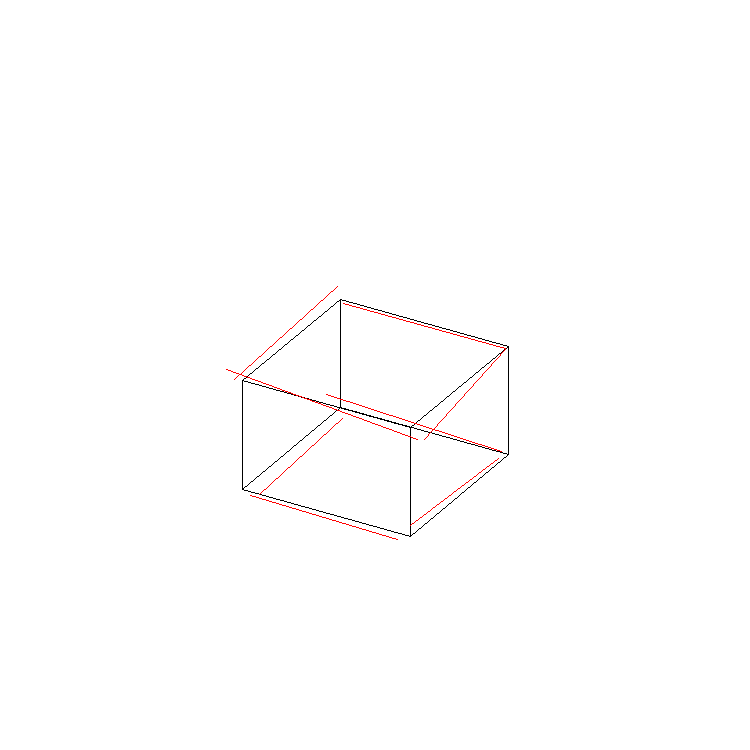
\includegraphics[width=0.5\textwidth]{variant2/images/1/input.png} &
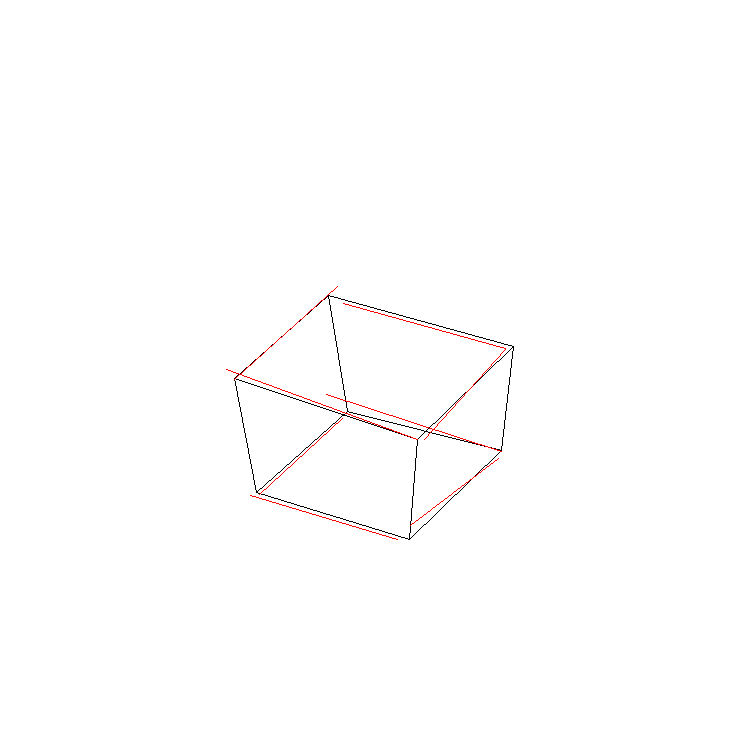
\includegraphics[width=0.5\textwidth]{variant2/images/1/out.png} \\
\midrule
\multicolumn{2}{|c|}{ 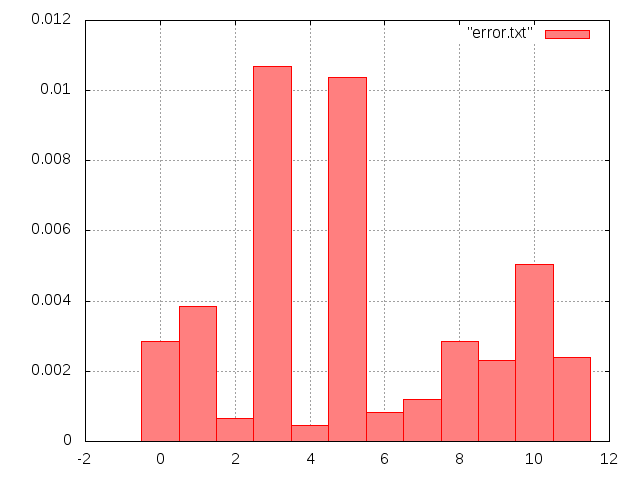
\includegraphics[width=0.8\textwidth]{variant2/images/1/error.png}} \\
\hline
\end{tabular}
\end{center}

\begin{center}

\begin{tabular}{|c|c|}
\hline
The original polyhedron& Rebuilt polyhedron \\
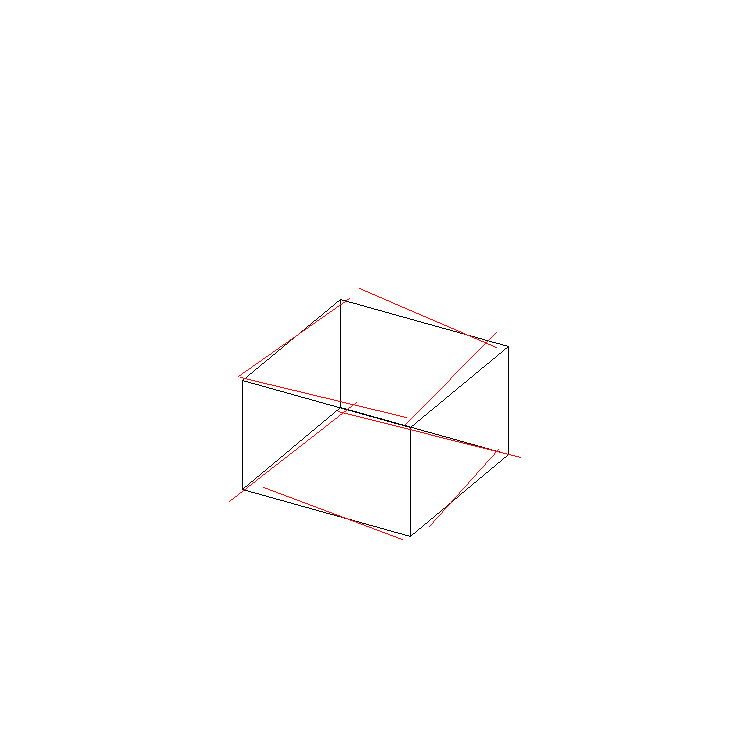
\includegraphics[width=0.5\textwidth]{variant2/images/2/input.png} &
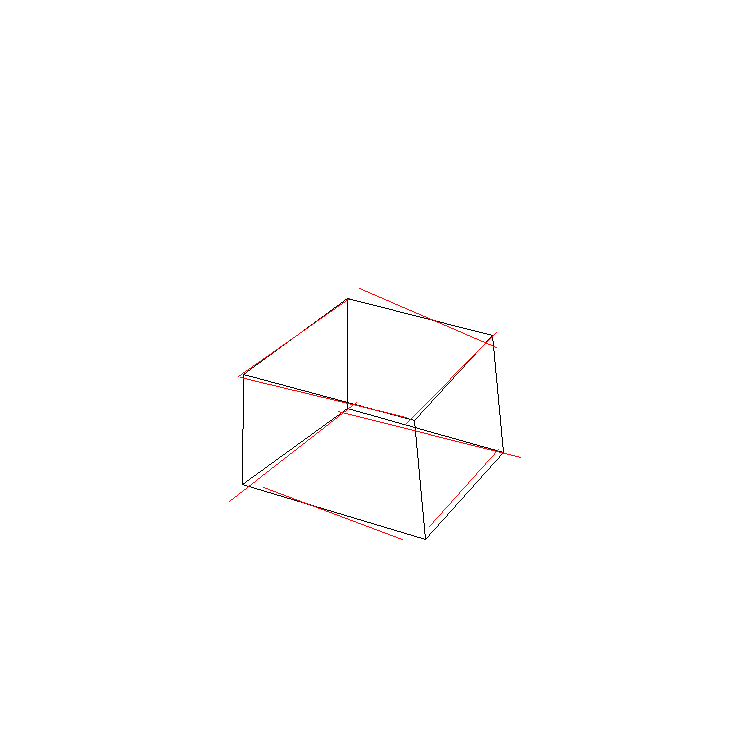
\includegraphics[width=0.5\textwidth]{variant2/images/2/out.png} \\
\midrule
\multicolumn{2}{|c|}{ 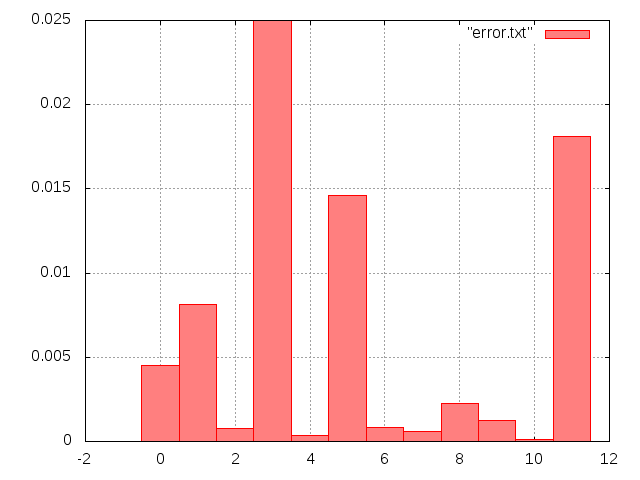
\includegraphics[width=0.8\textwidth]{variant2/images/2/error.png}} \\
\hline
\end{tabular}
\end{center}
\begin{center}

\begin{tabular}{|c|c|}
\hline
The original polyhedron& Rebuilt polyhedron \\
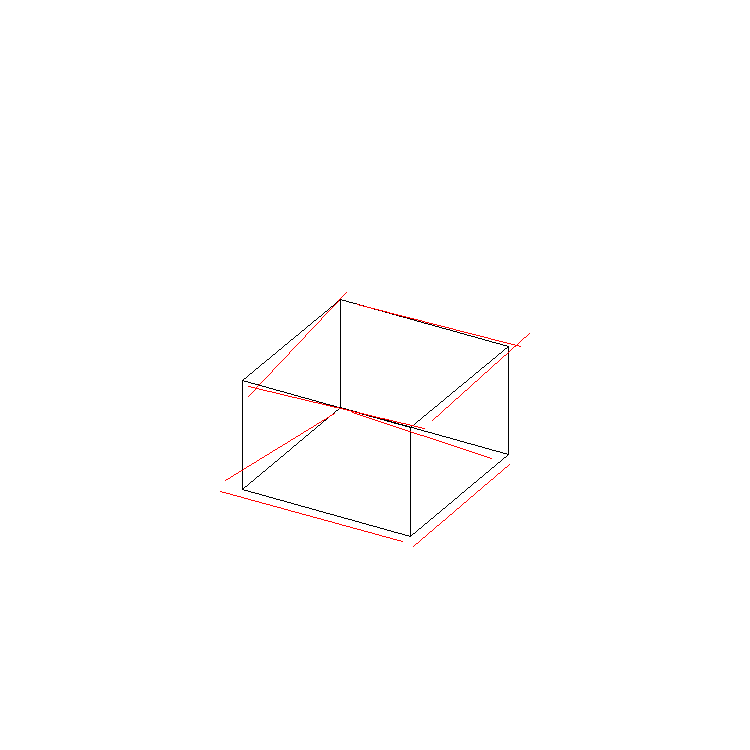
\includegraphics[width=0.5\textwidth]{variant2/images/3/input.png} &
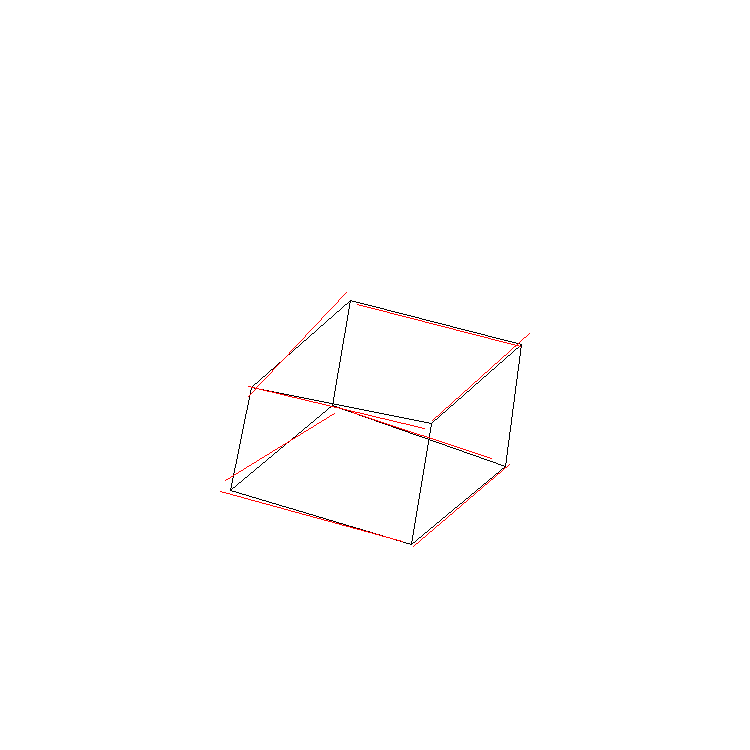
\includegraphics[width=0.5\textwidth]{variant2/images/3/out.png} \\
\midrule
\multicolumn{2}{|c|}{ 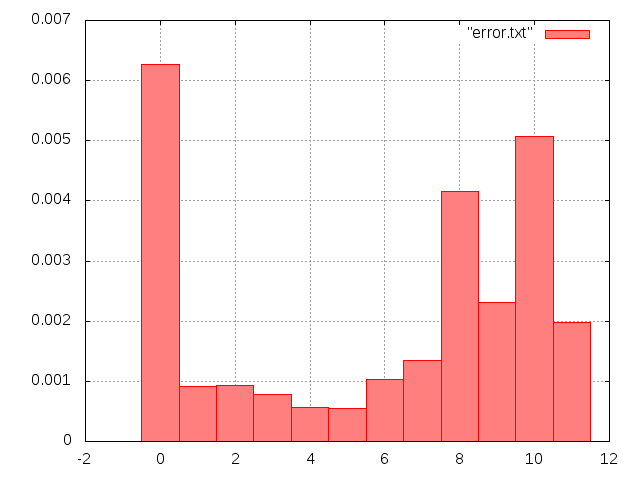
\includegraphics[width=0.8\textwidth]{variant2/images/3/error.png}} \\
\hline
\end{tabular}
\end{center}

\begin{center}

\begin{tabular}{|c|c|}
\hline
The original polyhedron& Rebuilt polyhedron \\
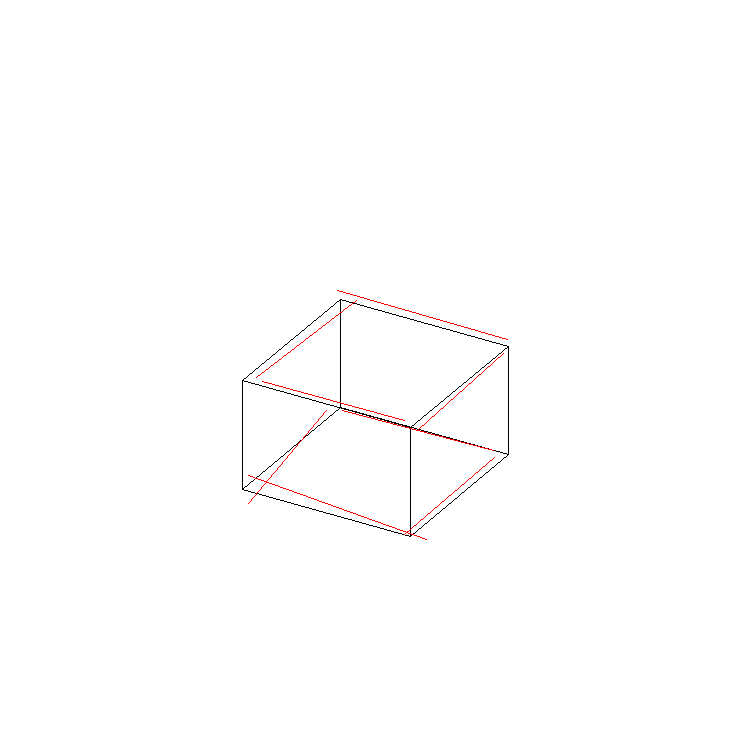
\includegraphics[width=0.5\textwidth]{variant2/images/4/input.png} &
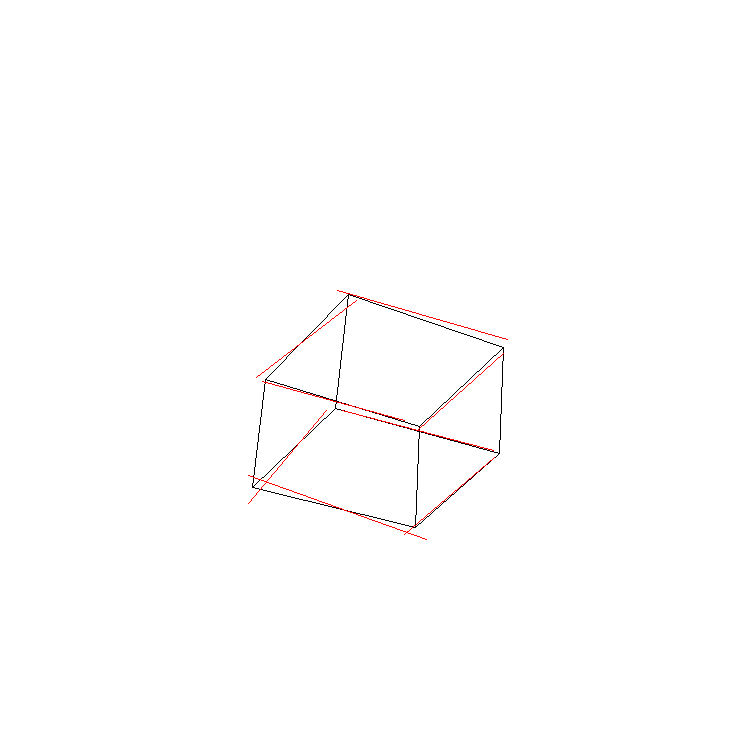
\includegraphics[width=0.5\textwidth]{variant2/images/4/out.png} \\
\midrule
\multicolumn{2}{|c|}{ 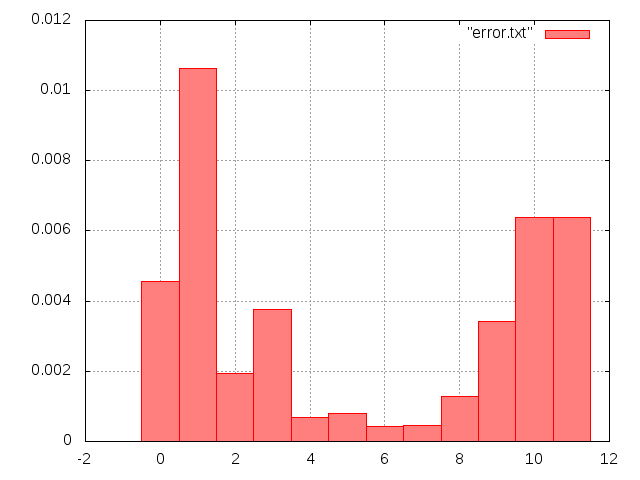
\includegraphics[width=0.8\textwidth]{variant2/images/4/error.png}} \\
\hline
\end{tabular}
\end{center}
\begin{center}

\begin{tabular}{|c|c|}
\hline
The original polyhedron& Rebuilt polyhedron \\
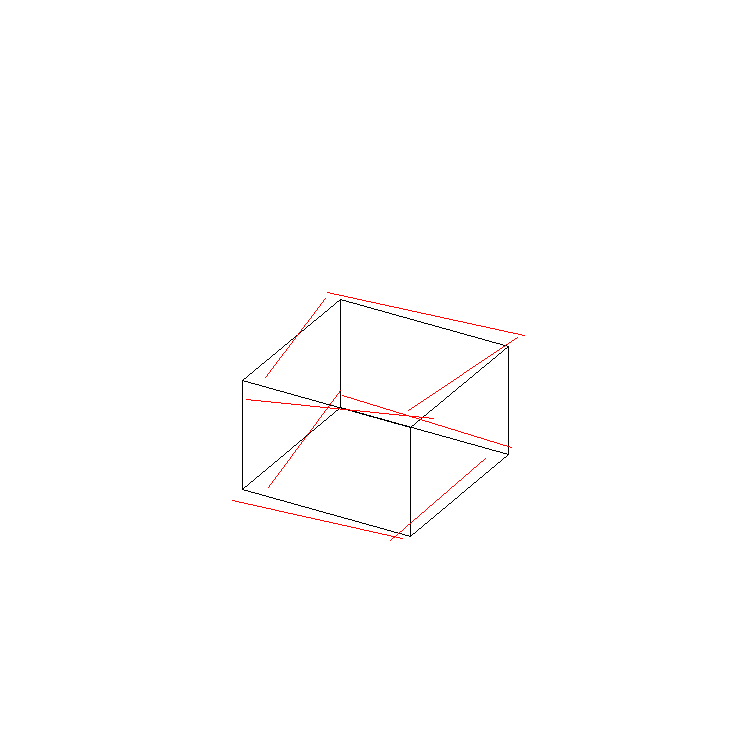
\includegraphics[width=0.5\textwidth]{variant2/images/5/input.png} &
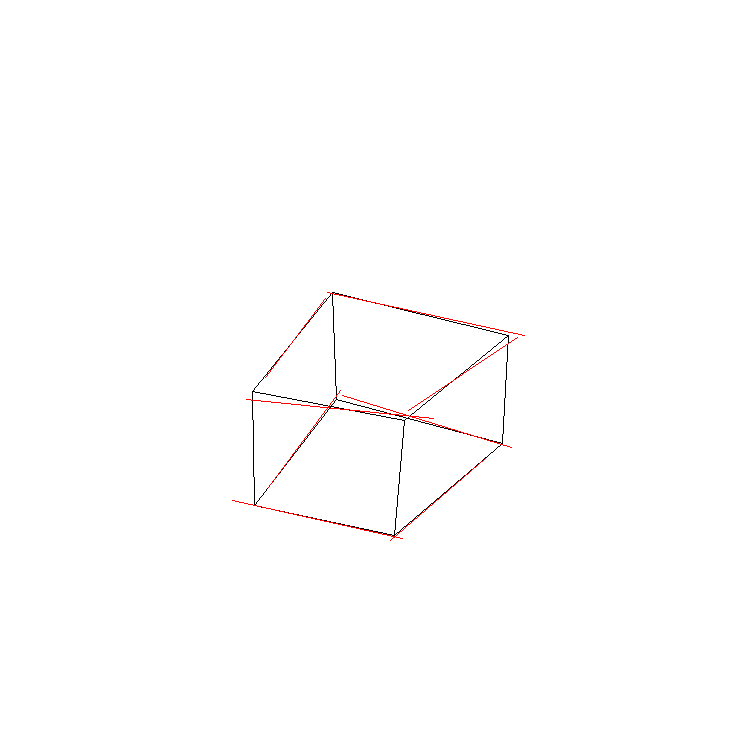
\includegraphics[width=0.5\textwidth]{variant2/images/5/out.png} \\
\midrule
\multicolumn{2}{|c|}{ 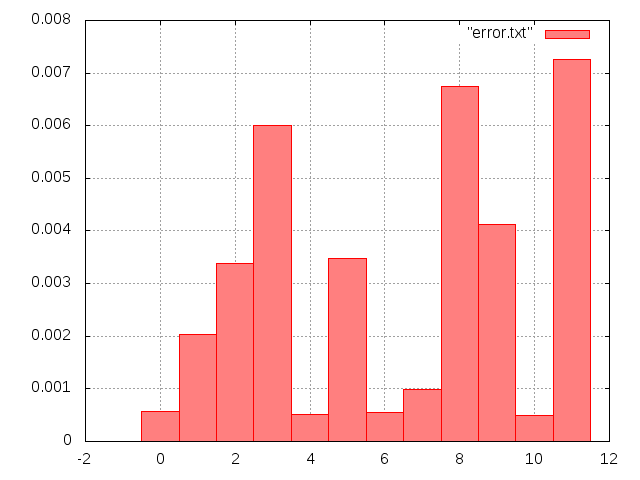
\includegraphics[width=0.8\textwidth]{variant2/images/5/error.png}} \\
\hline
\end{tabular}
\end{center}
\newpage
\subsubsection{Average deviations $|\Delta x_{i}|<0.25,|\Delta y_{i}|<0.25,|\Delta z_{i}|<0.25$}
\begin{center}

\begin{tabular}{|c|c|}
\hline
The original polyhedron& Rebuilt polyhedron \\
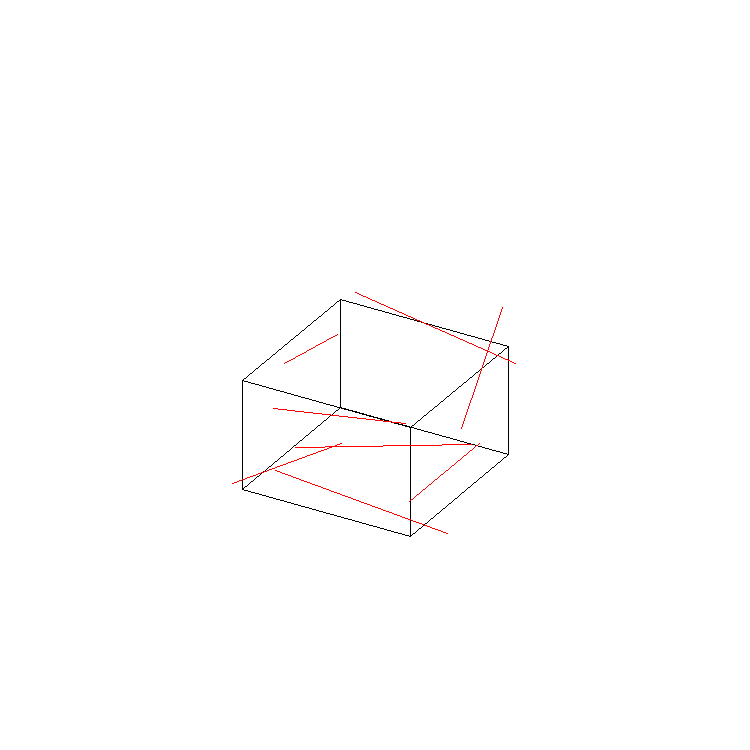
\includegraphics[width=0.5\textwidth]{variant2/images/21/input.png} &
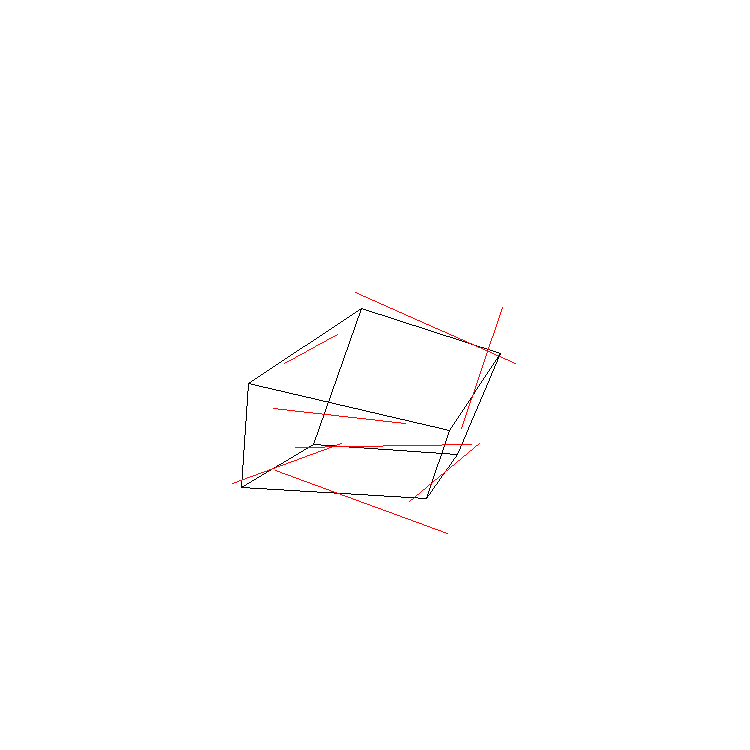
\includegraphics[width=0.5\textwidth]{variant2/images/21/out.png} \\
\midrule
\multicolumn{2}{|c|}{ 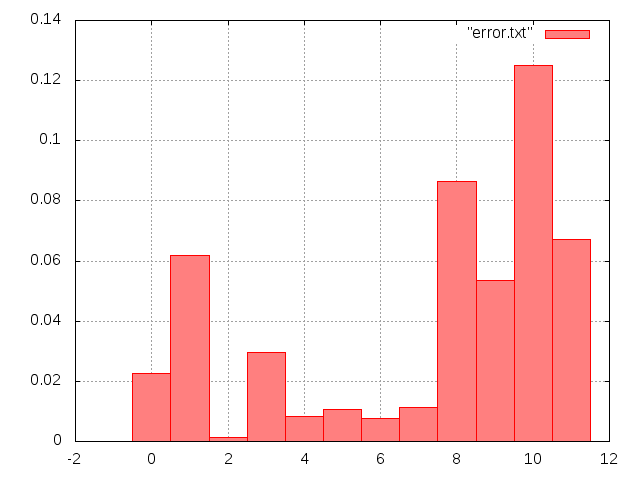
\includegraphics[width=0.8\textwidth]{variant2/images/21/error.png}} \\
\hline
\end{tabular}
\end{center}

\begin{center}

\begin{tabular}{|c|c|}
\hline
The original polyhedron& Rebuilt polyhedron \\
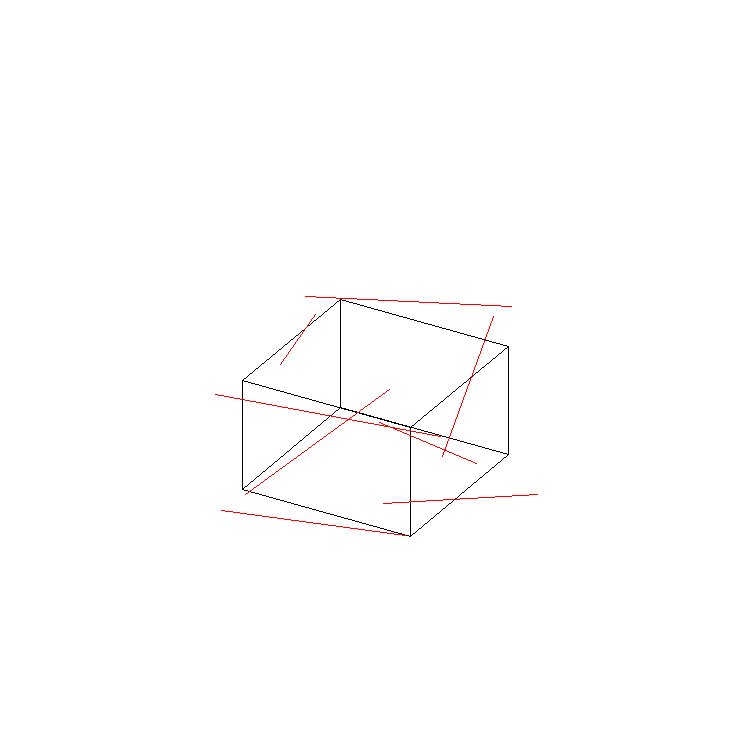
\includegraphics[width=0.5\textwidth]{variant2/images/22/input.png} &
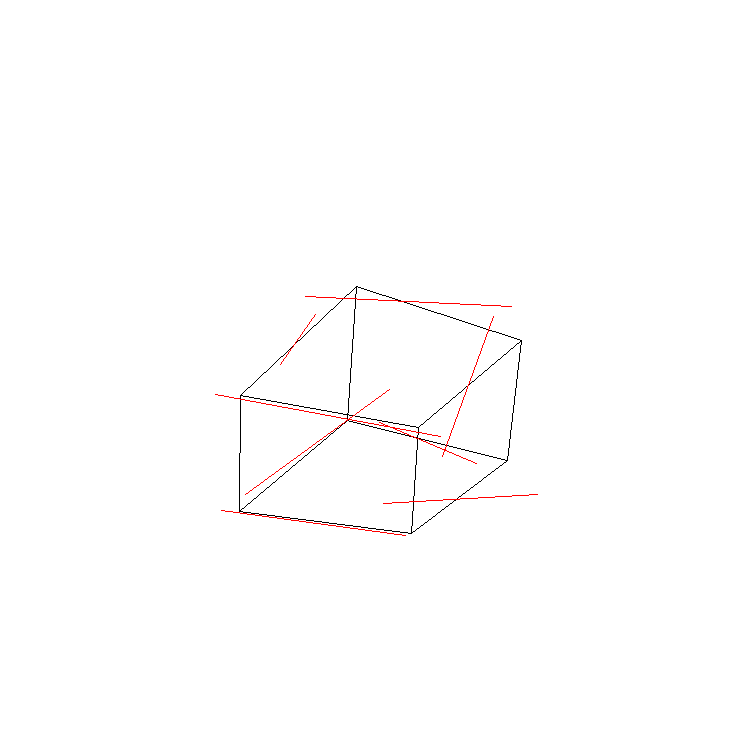
\includegraphics[width=0.5\textwidth]{variant2/images/22/out.png} \\
\midrule
\multicolumn{2}{|c|}{ 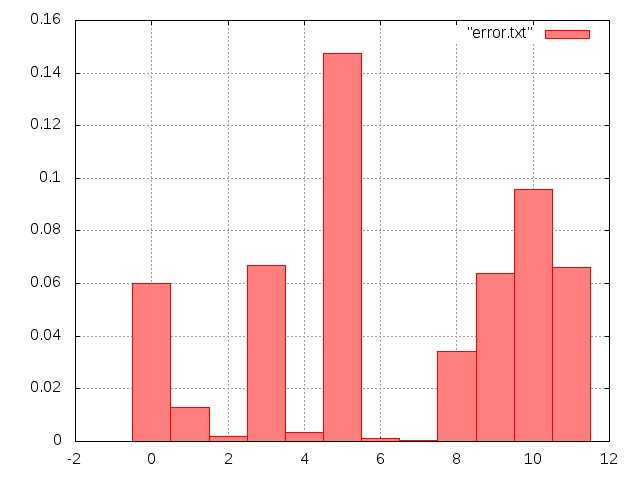
\includegraphics[width=0.8\textwidth]{variant2/images/22/error.png}} \\
\hline
\end{tabular}
\end{center}
\begin{center}

\begin{tabular}{|c|c|}
\hline
The original polyhedron& Rebuilt polyhedron \\
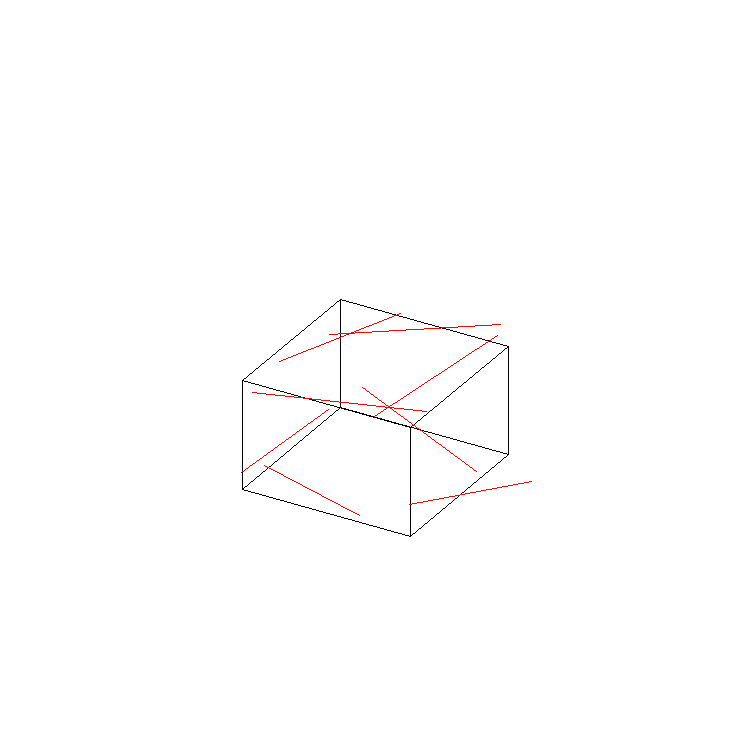
\includegraphics[width=0.5\textwidth]{variant2/images/23/input.png} &
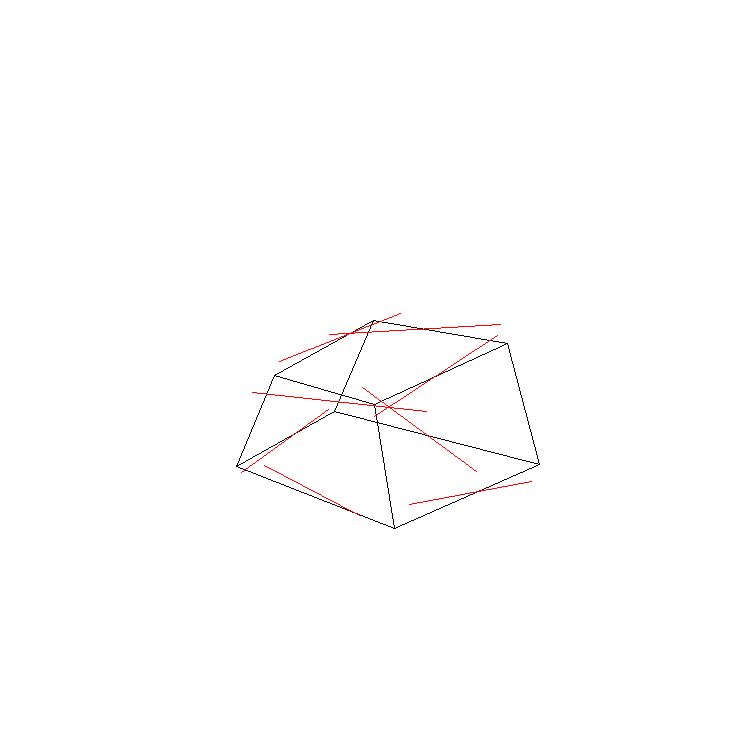
\includegraphics[width=0.5\textwidth]{variant2/images/23/out.png} \\
\midrule
\multicolumn{2}{|c|}{ 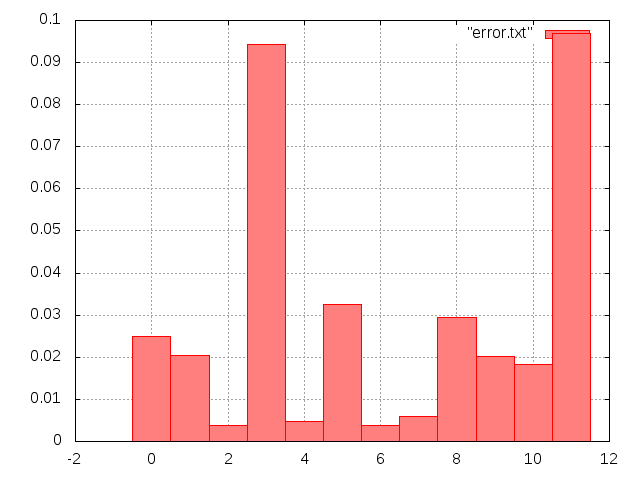
\includegraphics[width=0.8\textwidth]{variant2/images/23/error.png}} \\
\hline
\end{tabular}
\end{center}

\begin{center}

\begin{tabular}{|c|c|}
\hline
The original polyhedron& Rebuilt polyhedron \\
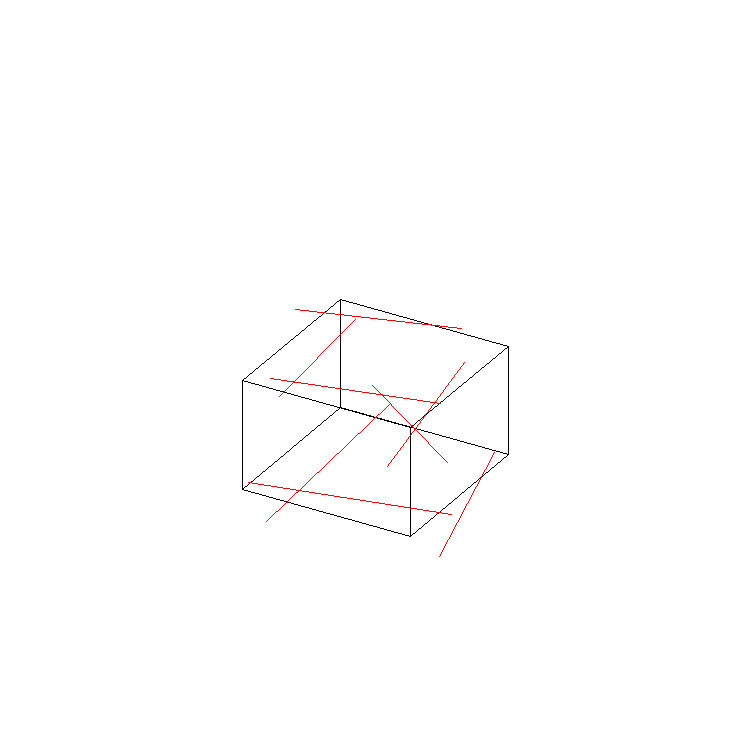
\includegraphics[width=0.5\textwidth]{variant2/images/24/input.png} &
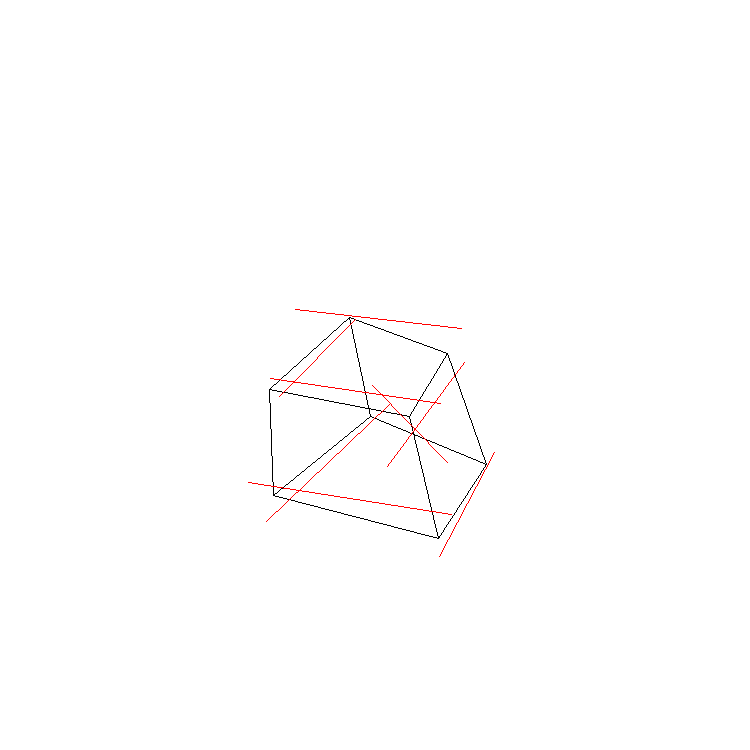
\includegraphics[width=0.5\textwidth]{variant2/images/24/out.png} \\
\midrule
\multicolumn{2}{|c|}{ 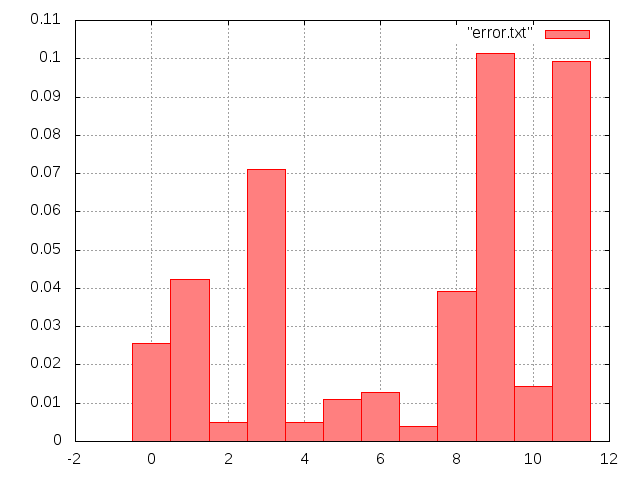
\includegraphics[width=0.8\textwidth]{variant2/images/24/error.png}} \\
\hline
\end{tabular}
\end{center}

\begin{center}

\begin{tabular}{|c|c|}
\hline
The original polyhedron& Rebuilt polyhedron \\
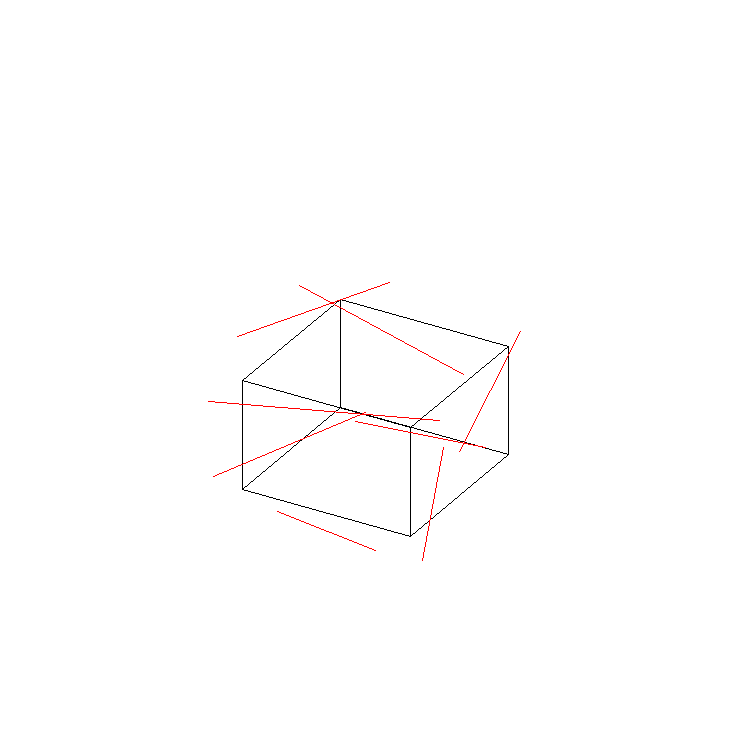
\includegraphics[width=0.5\textwidth]{variant2/images/25/input.png} &
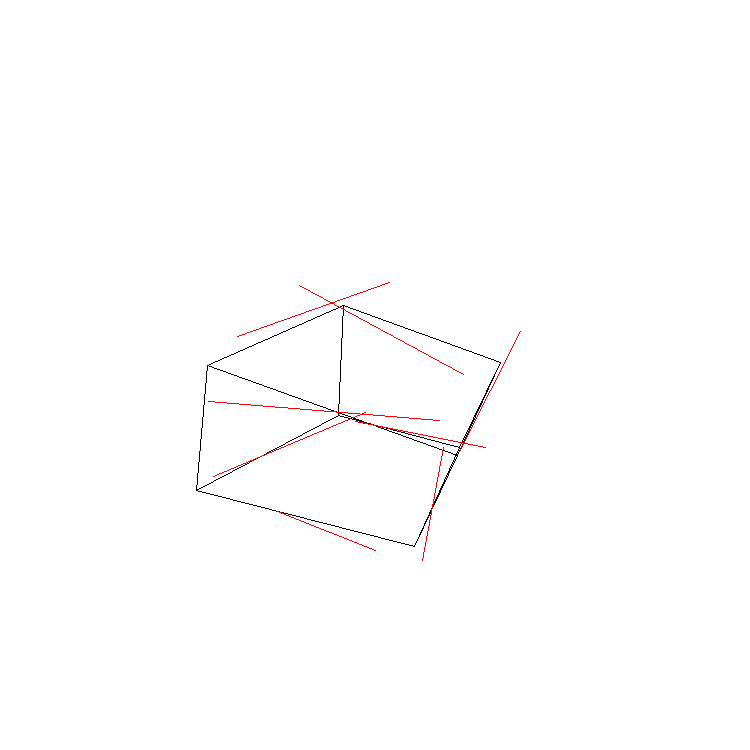
\includegraphics[width=0.5\textwidth]{variant2/images/25/out.png} \\
\midrule
\multicolumn{2}{|c|}{ 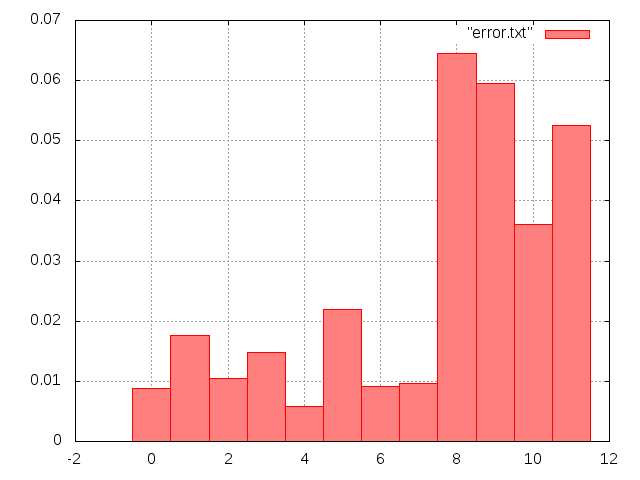
\includegraphics[width=0.8\textwidth]{variant2/images/25/error.png}} \\
\hline
\end{tabular}
\end{center}
\newpage
\subsubsection{Large deviations $|\Delta x_{i}|<0.5,|\Delta y_{i}|<0.5,|\Delta z_{i}|<0.5$}
\begin{center}

\begin{tabular}{|c|c|}
\hline
The original polyhedron& Rebuilt polyhedron \\
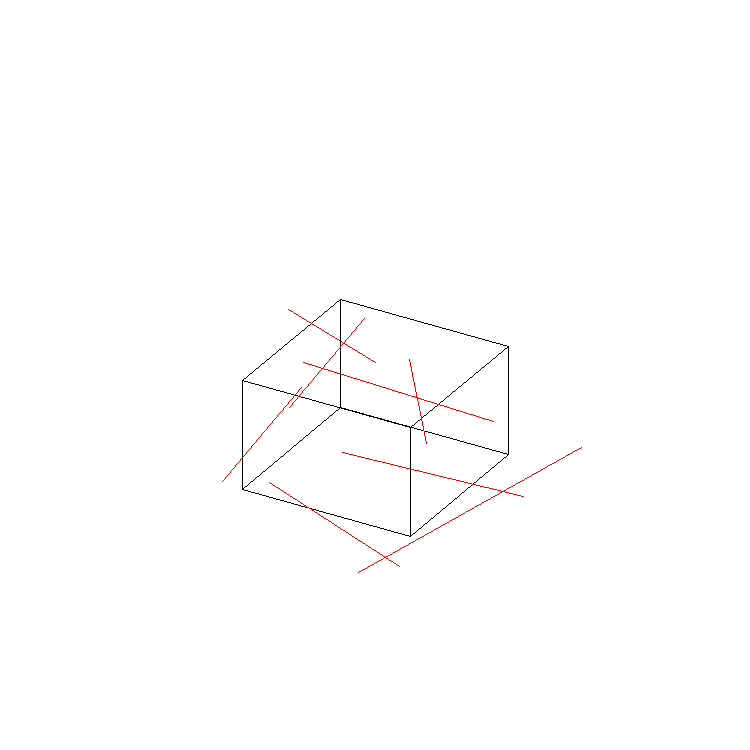
\includegraphics[width=0.5\textwidth]{variant2/images/11/input.png} &
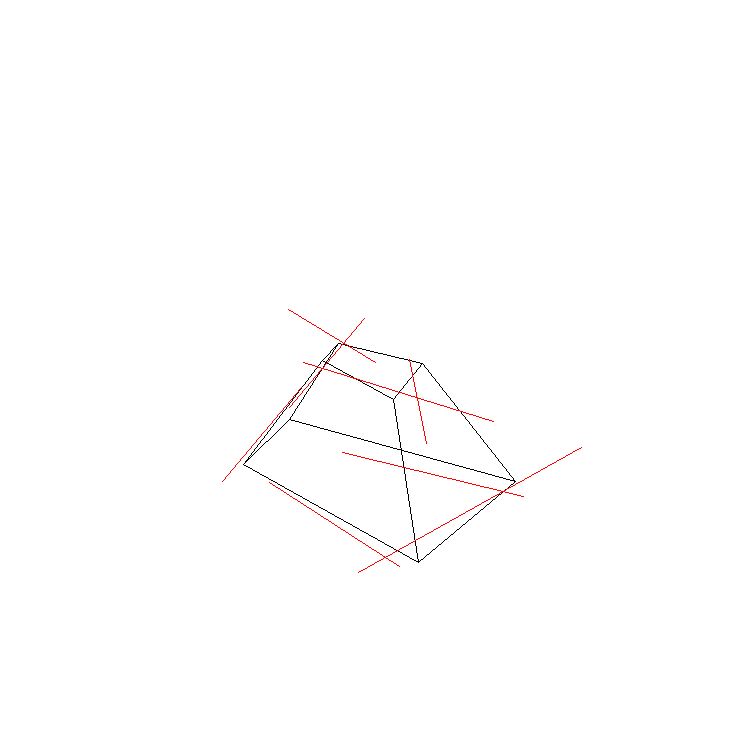
\includegraphics[width=0.5\textwidth]{variant2/images/11/out.png} \\
\midrule
\multicolumn{2}{|c|}{ 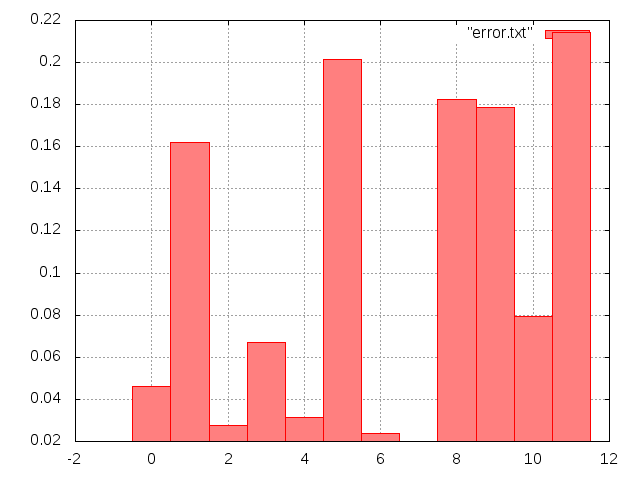
\includegraphics[width=0.8\textwidth]{variant2/images/11/error.png}} \\
\hline
\end{tabular}
\end{center}

\begin{center}

\begin{tabular}{|c|c|}
\hline
The original polyhedron& Rebuilt polyhedron \\
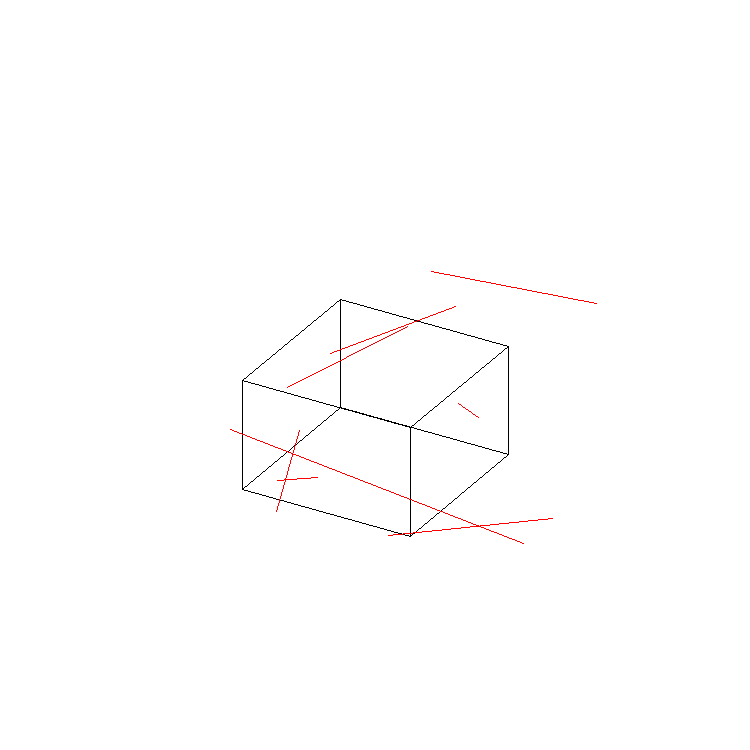
\includegraphics[width=0.5\textwidth]{variant2/images/12/input.png} &
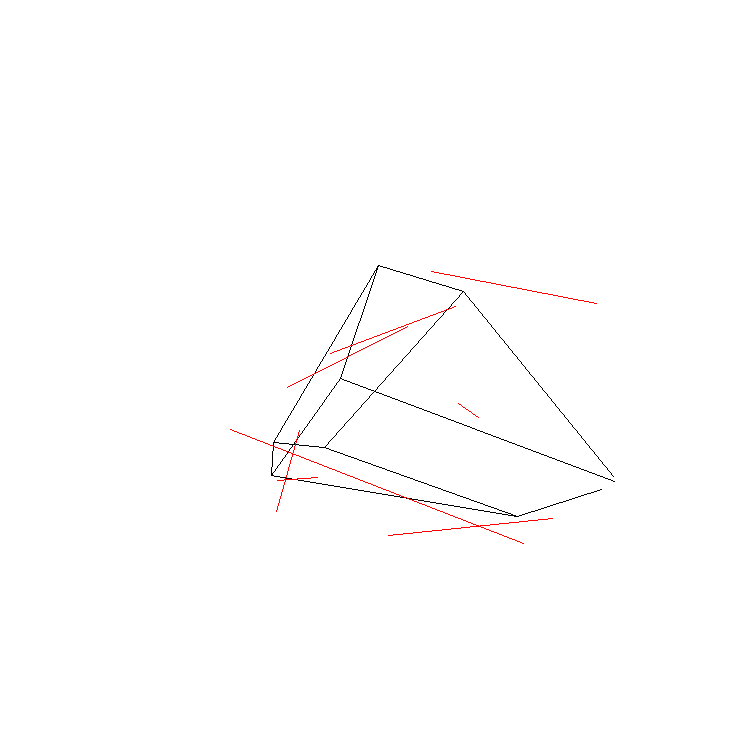
\includegraphics[width=0.5\textwidth]{variant2/images/12/out.png} \\
\midrule
\multicolumn{2}{|c|}{ 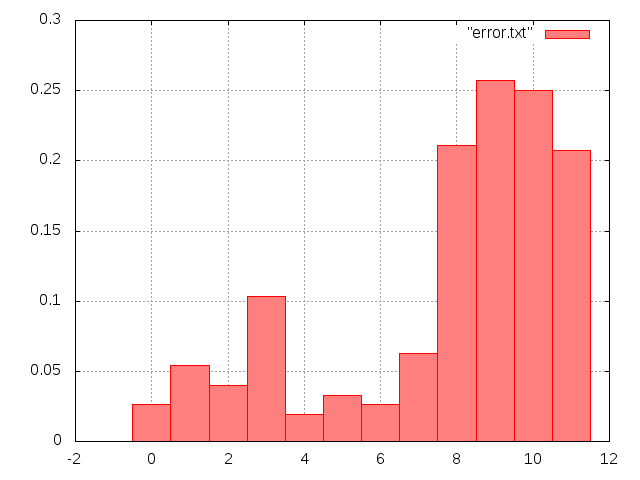
\includegraphics[width=0.8\textwidth]{variant2/images/12/error.png}} \\
\hline
\end{tabular}
\end{center}
\begin{center}

\begin{tabular}{|c|c|}
\hline
The original polyhedron& Rebuilt polyhedron \\
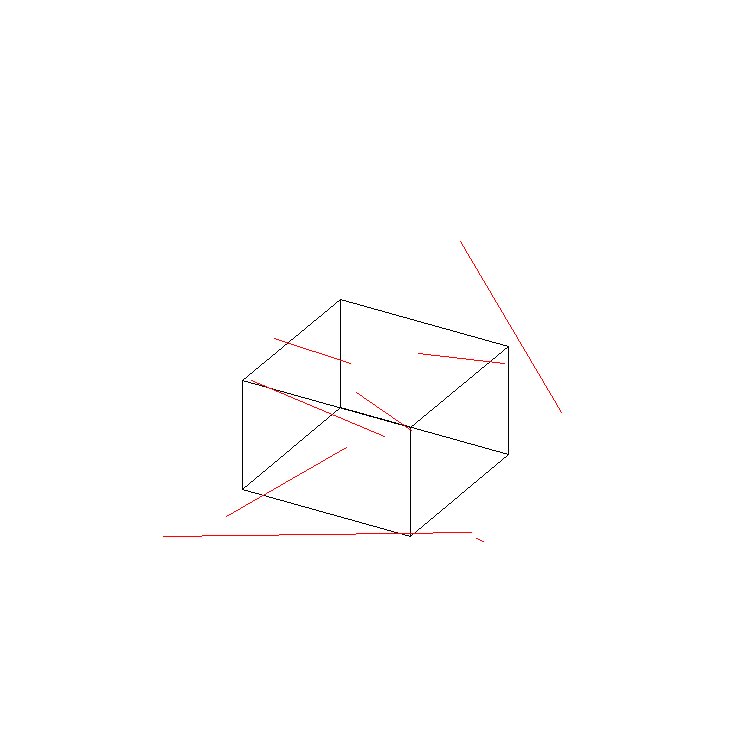
\includegraphics[width=0.5\textwidth]{variant2/images/13/input.png} &
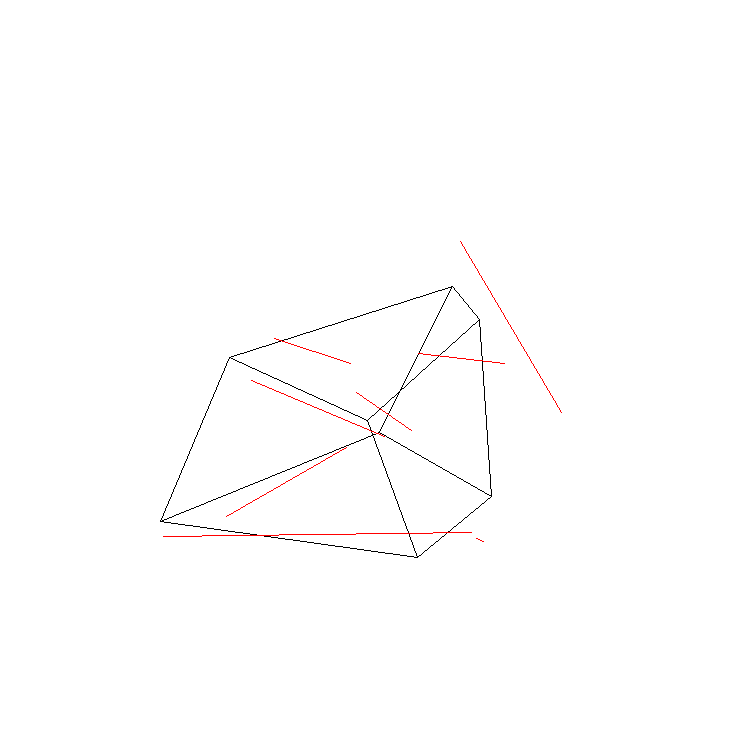
\includegraphics[width=0.5\textwidth]{variant2/images/13/out.png} \\
\midrule
\multicolumn{2}{|c|}{ 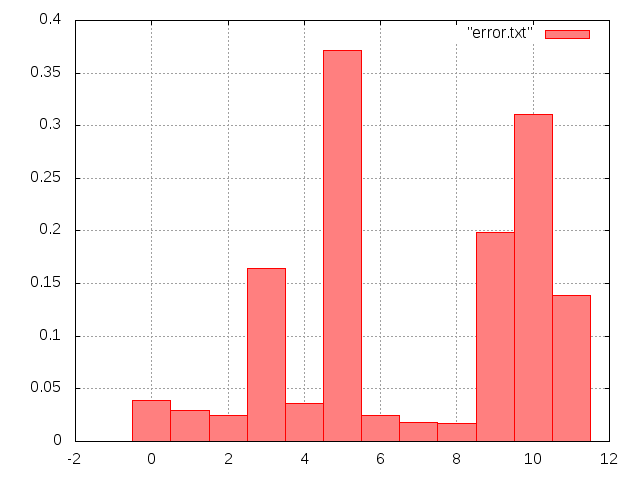
\includegraphics[width=0.8\textwidth]{variant2/images/13/error.png}} \\
\hline
\end{tabular}
\end{center}

\begin{center}

\begin{tabular}{|c|c|}
\hline
The original polyhedron& Rebuilt polyhedron \\
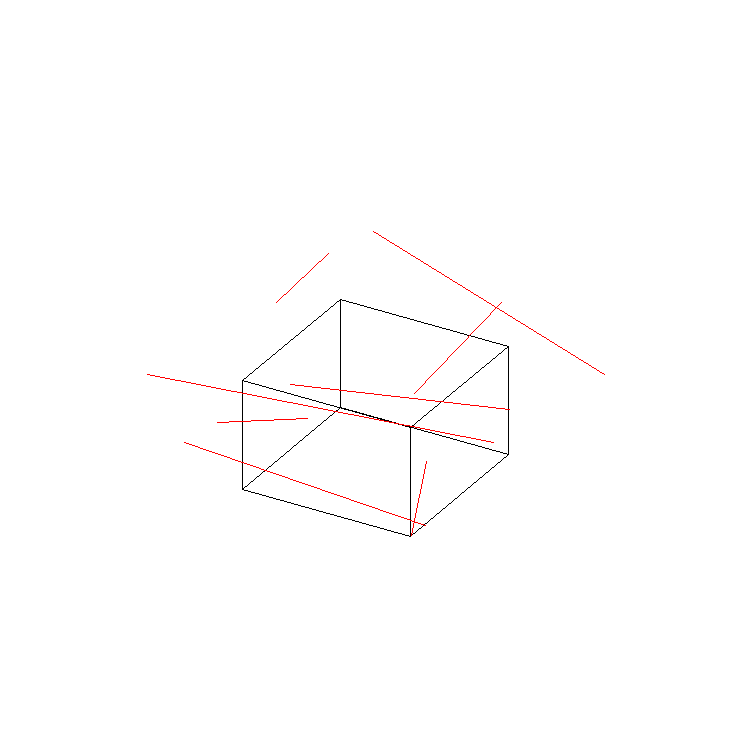
\includegraphics[width=0.5\textwidth]{variant2/images/14/input.png} &
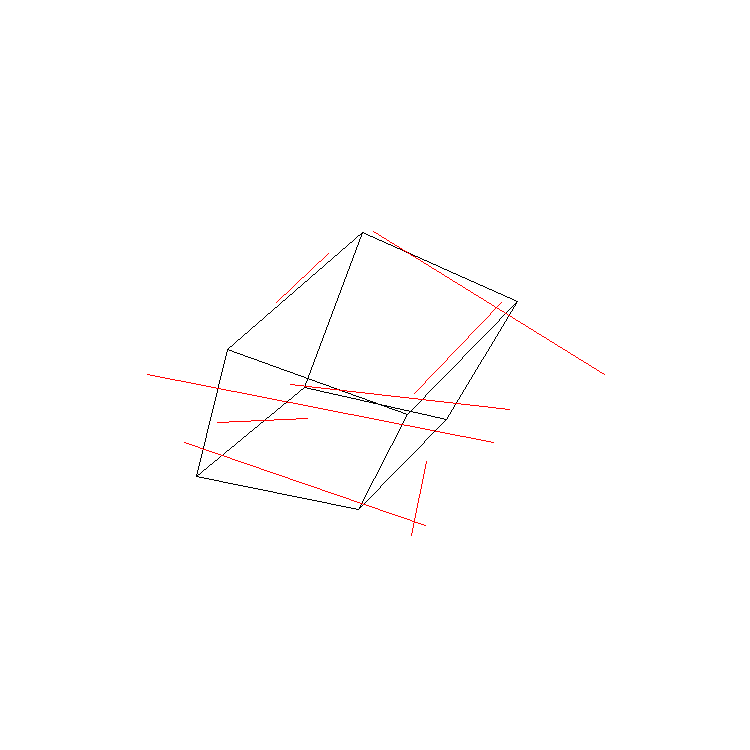
\includegraphics[width=0.5\textwidth]{variant2/images/14/out.png} \\
\midrule
\multicolumn{2}{|c|}{ 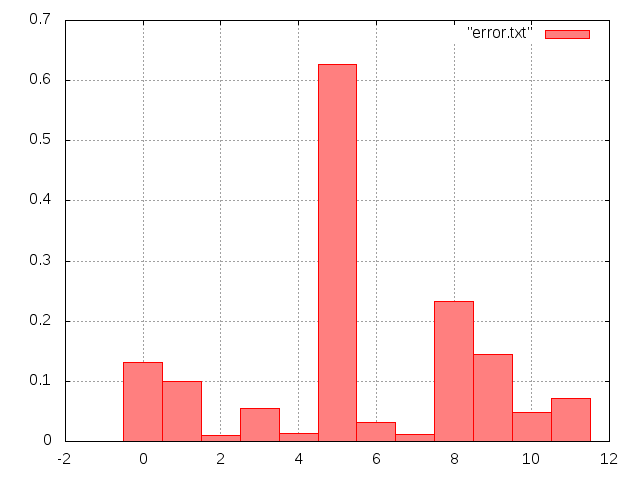
\includegraphics[width=0.8\textwidth]{variant2/images/14/error.png}} \\
\hline
\end{tabular}
\end{center}

\begin{center}

\begin{tabular}{|c|c|}
\hline
The original polyhedron& Rebuilt polyhedron \\
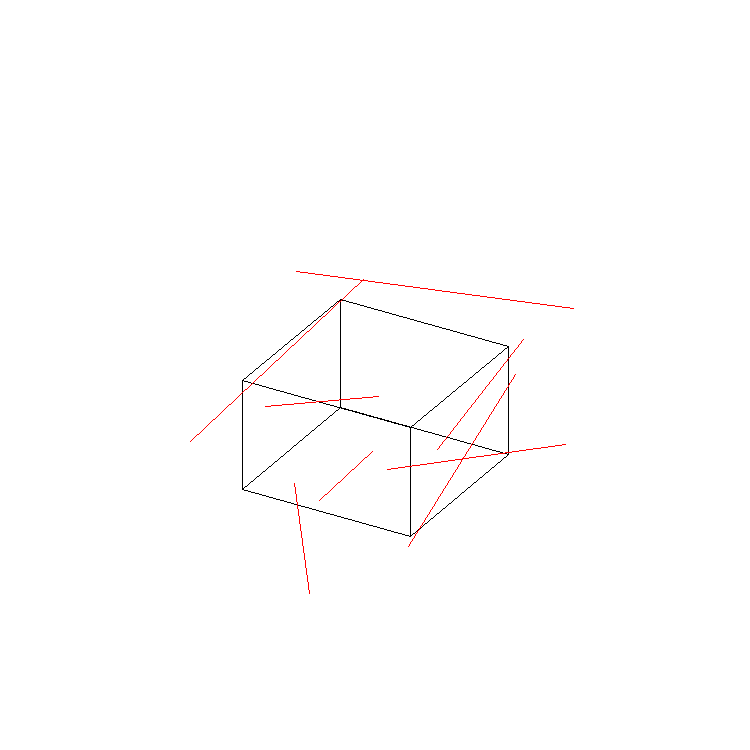
\includegraphics[width=0.5\textwidth]{variant2/images/15/input.png} &
\includegraphics[width=0.5\textwidth]{variant2/images/15/out.png} \\
\midrule
\multicolumn{2}{|c|}{ \includegraphics[width=0.8\textwidth]{variant2/images/15/error.png}} \\
\hline
\end{tabular}
\end{center}
\newpage
\subsection{The first test of the polyhedron.}
\begin{center}
\begin{tabular}{|c|c|}
\hline
Reconstructed polyhedron & Error on the ribs\\
\includegraphics[width=0.5\textwidth]{bigout1.png} &
\includegraphics[width=0.5\textwidth]{bigerror1.png} \\
\hline
\end{tabular}
\end{center}
\textbf{The value of the functional:} $3.9*10^{-4}$\\
\textbf{Operating time:} $405$ seconds\\
\textbf{number of iterations:} $478$\\
\textbf{number of vertexes:} $442$\\
\textbf{the Number of edges:} $663$\\
\textbf{the Number of faces:} $223$\\
\textbf{Number of target edges:} $35$ \\
\textbf{the Number of variables:} $4870$\\
\textbf{Number of non-zero elements in the Jacobian:} $9951$\\
\newpage
\subsection{The second test of the polyhedron.}
\begin{center}
\begin{tabular}{|c|c|}
\hline
Reconstructed polyhedron & Error on the ribs\\
\includegraphics[width=0.5\textwidth]{bigout2.png} &
\includegraphics[width=0.5\textwidth]{bigerror2.png} \\
\hline
\end{tabular}
\end{center}
\textbf{The value of the functional:} $7.6*10^{-4}$\\
\textbf{Operating time:} $635$ seconds\\
\textbf{number of iterations:} $526$\\
\textbf{number of vertexes:} $536$\\
\textbf{the Number of edges:} $804$\\
\textbf{the Number of faces:} $270$\\
\textbf{Number of target edges:} $68$ \\
\textbf{the Number of variables:} $5904$\\
\textbf{Number of non-zero elements in the Jacobian:} $12066$\\
\section{Speed up work on large models.}
Unfortunately, the algorithm takes a long time to work on large models. However, from the error histograms, you can see that on more than half of the edges, the distance from the target edges is zero. These are the edges of the lower part of the crystal, for which there are initially no target edges and they are attracted to themselves. As a result, they are static and their movement does not occur, but their movement is calculated. We will now include only edges in the functional that lie in faces that include at least one target edge. This model is somewhat more difficult to program, but it will speed up ten times. So the first crystal approaches in 10 seconds after 37 iterations, and the second-in 20 seconds after 41 iterations.
\newpage
\begin{thebibliography}{5}
\bibitem{1}
Веселов А. П., Троицкий Е. В. Лекции по аналитической геометрии. Учебное пособие. –– Изд. новое. –– М.: МЦНМО, 2016. –– 152 с. 
\bibitem{2}
Алексеев В.М., Галеев Э.М., Тихомиров В.М. Сборник задач по оптимизации. Теория. Примеры. Задачи: Учеб. пособие. --- 2-е изд. М.: ФИЗМАТЛИТ, 2005. --- 256 с.
\bibitem{3}
О.А. Щербина КРАТКОЕ ВВЕДЕНИЕ В AMPL - CОВРЕМЕННЫЙ АЛГЕБРАИЧЕСКИЙ ЯЗЫК МОДЕЛИРОВАНИЯ (препринт), 2012. --- 29 c. 
\bibitem{4}
Попов А.В. GNUPLOT и его приложения. --- М.: Издательство попечительского совета механико-математического факультета МГУ, 2015 , ---240 с. 
\bibitem{5} Introduction to Ipopt: A tutorial for downloading, installing, and using Ipopt. July 20, 2016
\end{thebibliography}
\end{document}